\documentclass[times, utf8, zavrsni, numeric]{fer}
\usepackage{booktabs}
\usepackage[hidelinks]{hyperref}
\usepackage{graphicx}
\usepackage{bm}
\usepackage{amsmath}
\usepackage{listings}
\usepackage{array}

\renewcommand{\lstlistingname}{Programski isječak}% Listing -> Algoritam
\renewcommand{\lstlistlistingname}{Popis programskih isječaka}% List of Listings -> Popis algoritama
 
\lstdefinestyle{mystyle} {
    basicstyle=\footnotesize,
    numbers=left,
    numberstyle=\tiny,
    frame=tb,
    columns=fullflexible,
    showstringspaces=false
    breakatwhitespace=false,        
    breaklines=true,                
    captionpos=b,                    
    keepspaces=true,                
    numbersep=5pt,                  
    showspaces=false,                
    showtabs=false,                  
    tabsize=4,
    inputencoding=utf8,
    morekeywords={vrati, ako, inače, za\_svaku, za\_svaki, prekini\_petlju, dok, funkcija}
}  
 
\lstset{style=mystyle,texcl=true}
% set font translations
%\lstset{inputencoding=utf8}
\lstset{extendedchars=true}
\lstset{
    literate=%
    {ć}{{\'c}}1
    {č}{{\v{c}}}1
    {đ}{{\dj{}}}1
    {š}{{\v{s}}}1
    {ž}{{\v{z}}}1
    {Ć}{{\'C}}1
    {Č}{{\v{C}}}1
    {Đ}{{\DJ{}}}1
    {Š}{{\v{S}}}1
    {Ž}{{\v{Z}}}1
}

\newcommand{\matr}[1]{\mathbf{#1}}
\newcommand{\hiperravnina}{$\langle \mathbf{w}, b \rangle$}
\newcommand{\iteralpha}{\boldsymbol{\alpha}_i^{k}}
\newcolumntype{L}[1]{>{\raggedright\let\newline\\\arraybackslash\hspace{0pt}}m{#1}}

\interfootnotelinepenalty=10000

\graphicspath{{"D:/fer/6. semestar/ZAVRAD/svm-sentiment-analysis/Thesis/Slike/"}}

\begin{document}

% TODO: Navedite broj rada.
\thesisnumber{5179}

% TODO: Navedite naslov rada.
\title{Primjena stroja s potpornim vektorima za analizu sentimenta korisničkih recenzija}

% TODO: Navedite svoje ime i prezime.
\author{Dominik Stanojević}

\maketitle

% Ispis stranice s napomenom o umetanju izvornika rada. Uklonite naredbu \izvornik ako želite izbaciti tu stranicu.
\izvornik

% Dodavanje zahvale ili prazne stranice. Ako ne želite dodati zahvalu, naredbu ostavite radi prazne stranice.
\zahvala{}

\tableofcontents

\chapter{Uvod}

\par Klasifikacijski i regresijski problemi jedni su od najvažnijih problema strojnog učenja. 
Modeli poput linearne i logističke regresije pogodni su za jednostavnije probleme.
Zahvaljujući sve većoj dostupnosti podataka i povećanju procesorske moći današnjih računala,
pojavljuju se složeniji zadaci za koje navedene metode nisu efikasne.

\par Pojava složenijih zadataka rezultirala je i pojavom složenijih metoda koje mogu doskočiti 
istima. Modeli poput slučajnih šuma i modeli iz skupine dubokog učenja u mogućnosti su rješavati i složenije, 
nelinearne probleme.

\par Osim navedenih modela, još jedan model koji je sposoban efikasno obraditi nelinearne podatke 
je \textbf{stroj s potpornim vektorima} (engl. \textit{Support Vector Machine}, u nastavku SVM).
Koristeći jezgreni trik, stroj s potpornim vektorima uspješno razdvaja linearno nerazdvojive podatke.
Iako su temeljne ideje modela predstavljene prije više od pola stoljeća, stroj s potpornim vektorima i danas je jedan od
najrobusnijih modela za klasifikaciju i regresiju.

\par Jedan od zanimljivih problema koji dobro prikazuje robusnost SVM-a je \textbf{analiza sentimenta}
(engl. \textit{Sentiment Analysis}).
Subjektivnost emocija, kontekst te velika količina podataka svakako predstavljaju izazove u rješavanju problema.
Koristeći SVM, uz uvjet kvalitetnog pretprocesiranja podataka, mogu se postići zavidni rezultati u polju analize sentimenta.

\par U radu je predstavljen model stroja s potpornim vektorima te problem analize sentimenta.
U poglavlju \ref{ppodrucja} bit će predstavljen pregled područja, povijest modela stroja s potpornim vektorima te problem analize sentimenta.
U poglavlju \ref{svm} detaljnije će se obraditi model SVM.
Bit će opisana motivacija i interpretacija modela.
Nadalje, detaljnije će se pojasniti algoritmi optimizacije modela.
U poglavlju \ref{sentiment} formalizirat će se problem analize sentimenta.
Prikazat će se postupak pretprocesiranja podataka koji će podatke pretvoriti u oblik razumljiv SVM-u.
U petom poglavlju, provest će se eksperiment analize korisničkih recenzija uporabom opisanih metoda.
Ukratko će se analizirati dobiveni rezultati.
Poglavlje \ref{zakljucak} sadrži zaključak i ideje za daljnje istraživanje. 

\chapter{Pregled područja} \label{ppodrucja}
Godina začetka ideje modela stroja s potpornim vektorima može se smatrati 1963. kada sovjetski 
matematičar Vladimir Vapnik zajedno s Aleksandrom Lernerom izdaje publikaciju u kojoj je opisan
algoritam generaliziranog portreta (engl. \textit{Generalized Portrait Algorithm} \cite{vapnik1963}). 
Stroj s potpornim vektorima smatra se nelinearnom generalizacijom upravo tog algoritma.
Godinu kasnije Aizerman, Rozonoer i Braverman uvode pojam jezgrenih trikova \cite{Aizerman67theoretical}.
Corver 1965. godine iznosi ideju optimalno razdvajajućih hiperravnina \cite{cover1965browse}.
1992. godine objavljuje se rad u kojem se izlaže model stroja s potpornim vektorima koji je veoma
blizak današnjem modelu \cite{Boser:1992:TAO:130385.130401}.
Jedna od najvažnijih godina za model SVM je 1995. kada je riješen problem razdvajanja linearno 
nerazdvojivih podataka. Iste godine razvija se model stroja s potpornim vektorima za primjenu na regresijske 
probleme \cite{Cortes:1995:SN:218919.218929}.

\par U novijoj literaturi, model stroja s potpornim vektorima dobro je opisan u knjizi 
\textit{Elements Of Statistical Learning} \cite{hastie01statisticallearning} i materijalima s predavanja
sveučilišta Stanford \cite{NgSVM}.

\par Za razliku od modela stroja s potpornim vektorima koji je star već nekoliko desetljeća, 
problem analize sentimenta je relativno novi problem.
Izraz \textit{analiza sentimenta} prvi put se pojavljuje 2003. godine 
\cite{Nasukawa:2003:SAC:945645.945658}.
Sama ideja analize sentimenta pojavila se nešto ranije \cite{Pang+Lee+Vaithyanathan:02a}, 
\cite{wiebe-bruce-o'hara:1999:ACL}.
Područje analize sentimenta jedno je od najpopularnijih problema prirodnog jezika te se nova otkrića
i ideje javljaju gotovo svakodnevno. Jedna od najboljih uvodnih knjiga za ovaj problem je svakako
knjiga \textit{Sentiment Analysis and Opinion Mining} autora Bing Liu \cite{Liu:2012:SAO:3019323}.



\chapter{Stroj s potpornim vektorima} \label{svm}
U ovom poglavlju bit će predstavljen model stroja s potpornim vektorima. 
Potpoglavlje \ref{klasifikacija} definira pojam klasifikacije i pojašnjava razliku između klasifikacije i regresije.
U potpoglavlju \ref{hmargine} pojasnit će se ideja razdvajajuće hiperravnine.
Potpoglavlje \ref{margina} predstavit će pojam margine razdvajajuće hiperravnine i njenu važnost u izgradnji
klasifikatora.
Koristeći ideje iz prethodnih potpoglavlja, potpoglavlje \ref{opthiper} definira optimalnu razdvajajuću hiperravninu,
metodu koju koristi SVM prilikom klasifikacije podataka.
U potpoglavlju \ref{reg} daje se ideja regularizacije. Ova metoda omogućuje da stroj s potpornim vektorima
pronađe optimalnu hiperravninu u slučaju linearno nerazdvojivih podataka.
Potpoglavlja \ref{sec:primdual} i \ref{sec:svmopt} postavljaju primarni i dualni optimizacijski problem 
te koristeći dane ideje rješavaju problem optimizacije stroja s potpornim vektorima.
Potpoglavlje \ref{jezgra} opisuje transformaciju prostora značajki koristeći jezgrene trikove.
Jezgreni trikovi su efikasne metode koje omogućuju razdvajanje originalno linearno nerazdvojivih podataka.
Potpoglavlje \ref{sec:multiclass} posvećeno je metodama višerazredne klasifikacije koje omogućuju
klasifikaciju podataka s više od dva razreda.
U potpoglavlju \ref{sec:svr} proširuje se model stroja s potpornim vektorima za primjenu kod regresijskih
problema.


\section{Klasifikacija} \label{klasifikacija}
Problemi nadziranog učenja uobičajeno se dijele na dvije podskupine - klasifikaciju i regresiju.
Neka vektorski prostor $\textit{X}$ dimenzije $n$, primjerice $\mathbb{R}^n$, predstavlja skup primjeraka. 
Pojedini primjerak može se zadati vektorom: $\mathbf{x}=(x_1,x_2,\dots,x_n)$.
Ako pojedinom primjerku $\mathbf{x}$ pridružimo oznaku razreda $y$, tada se govori o \textbf{klasifikaciji}.
Pojednostavljeno, postupkom klasifikacije određuje se razred kojem određen primjerak $\mathbf{x}$ pripada.
Skup svih razreda $\textit{C}$ je konačan, a broj razreda dan je kardinalitetom $\left\vert{C}\right\vert$.

\begin{figure}
\centering
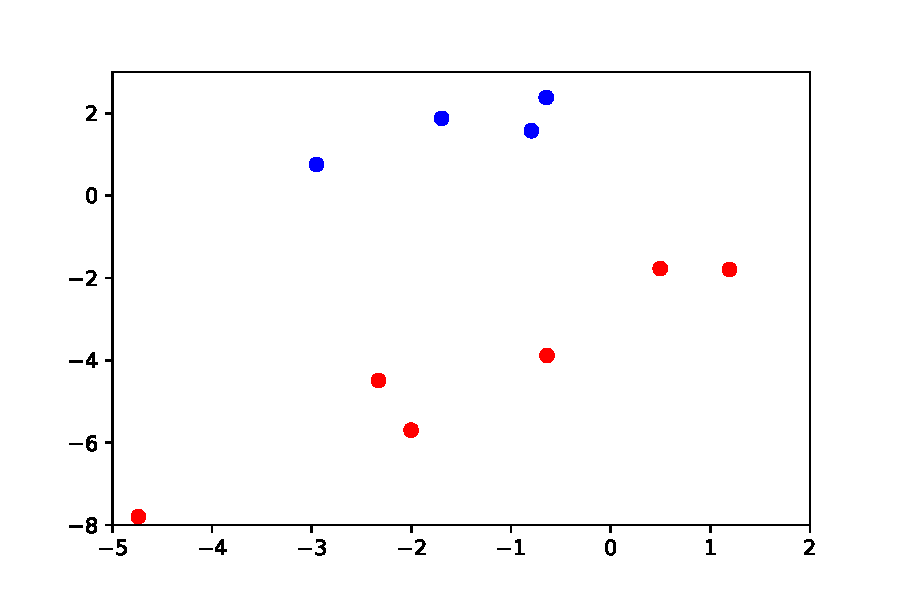
\includegraphics{klas.pdf}
\caption{Primjer klasifikacijskog problema}
\label{fig:klas}
\end{figure}


\par Primjer klasifikacijskog problema prikazan je slikom \ref{fig:klas}. 
Prostor primjeraka je $\mathbb{R}^2$, a skup razreda je dvočlani skup tj. $\left\vert{C}\right\vert=2$.
Klasifikacija podataka u dvočlane skupove naziva se \textbf{binarna klasifikacija}.
Upravo je stroj s potpornim vektorima primjer binarnog klasifikatora, no postoje metode koje pružaju mogućnost
višerazredne klasifikacije.
Osim gore navedenog primjera, još neki primjeri klasifikacije su otkrivanje neželjene pošte, prepoznavanje rukopisa,
prepoznavanje prometnih znakova, itd.

\par Za razliku od problema klasifikacije u kojem je varijabli $y$ pridružena vrijednost iz konačnog skupa, 
kod problema regresije primjerku pridružujemo vrijednost iz nekog beskonačnog skupa, primjerice $\mathbb{R}$.
Postoji modifikacija stroja s potpornim vektorima koji omogućuje rješavanje regresijskih problema.
Primjeri regresije su predviđanje iznosa plaće u ovisnosti o spolu, obrazovanju i sl., predviđanje broja prodanih 
primjeraka nekog prijenosnog računala, itd.

\section{Razdvajajuća hiperravnina} \label{hmargine}
Interpretaciju modela stroja s potpornim vektorima potrebno je započeti s pojmom koji nije strogo vezan uz sam model.
Primjerice model logističke regresije, iako temeljen na vjerojatnosti, u konačnici pronalazi hiperravninu kojom razdvaja
podatke.

\par Neka je zadan vektorski prostor $\textit{X}$ dimenzije $n$, primjerice $\mathbb{R}^n$.
Tada je \textbf{hiperravnina} definirana kao potprostor dimenzije $n-1$ unutar prostora $\textit{X}$.
Primjerice, u jednodimenzijskom prostoru hiperravnina je točka, u dvodimenzijskom prostoru
 hiperravninu predstavlja bilo koji pravac koji leži u ravnini, a u trodimenzijskom prostoru hiperravnina
 je predstavljena ravninom. 
Analogno, pojam hiperravnine vrijedi i za prostore većih dimenzija. 

\par Za hiperravninu zadanom izrazom $f(\mathbf{x})=b + \mathbf{w}^T\mathbf{x} = 0$ 
vrijede sljedeća svojstva:
\begin{enumerate}
  \item za svaku točku $T$ na hiperravnini vrijedi: $b = -\mathbf{w}^T\mathbf{x}$,
  \item jedinični vektor normale je zadan izrazom: $\mathbf{n} = \frac{\mathbf{w}}{\|\mathbf{w}\|}$,
  \item udaljenost točke $P$ od hiperravnine iznosi: $d = \frac{|f(\mathbf{x})|}{\|\mathbf{w}\|}$.
\end{enumerate}

Hiperravnina ovisi o vektoru težina $\mathbf{w}$ i slobodnom članu $b$. 
U daljnjem tekstu hiperravnina bit će zadana svojim parametrima, \hiperravnina{}. 

\par Hiperravnine same po sebi nisu pretjerano interesantne. 
No, za klasifikaciju interesantan je određen podskup hiperravnina.
Hiperravnina koja razdvaja dva razreda podataka naziva se \textbf{razdvajajuća hiperravnina.}
Uz pretpostavku $y \in \{-1, 1\}$, za razdvajajuću hiperravninu vrijedi:
\begin{equation}
  y^{(i)} = sgn(b + \mathbf{w}^T\mathbf{x}^{(i)}), \forall i
\end{equation}
gdje je $\mathbf{x}^{(i)}$ primjer iz skupa podataka, a $y^{(i)}$ je oznaka razreda pridružena primjeru $\mathbf{x}^{(i)}$.

\begin{figure}
\centering
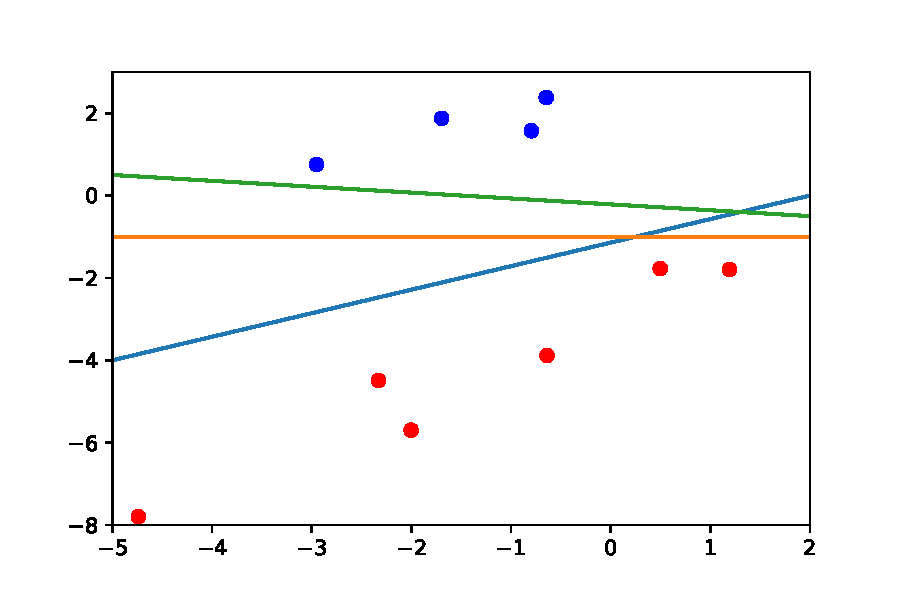
\includegraphics{hravnine.pdf}
\caption{Razdvajajuće hiperravnine}
\label{fig:hrav}
\end{figure}

Na slici \ref{fig:hrav} prikazani su primjerci jednaki onima sa slike \ref{fig:klas}.
Također, prikazane su i tri razdvajajuće hiperravnine. 
Valja primijetiti kako je moguće konstruirati beskonačno mnogo razdvajajućih hiperravnina.

\section{Margina razdvajajuće hiperravnine} \label{margina}
Za razliku od drugih klasifikatora koji traže bilo koju razdvajajuću hiperravninu kako bi klasificirali podatke,
stroj s potpornim vektorima uzima u obzir i udaljenosti primjeraka od hiperravnine. 
Intuitivno se može zaključiti kako je sigurnije odrediti razred za one primjerke koji su udaljeniji od 
hiperravnine. Udaljenost primjerka od hiperravnine nazivamo \textbf{margina}.

\par Neka je zadan $i$-ti primjerak $(\mathbf{x}^{(i)}, y^{(i)})$ gdje je $\mathbf{x}^{(i)}$ vektor značajki, 
a $y^{(i)}$ pripadajuća oznaka razreda.
Također, neka je $\mathbf{r^{(i)}}$ radij-vektor točke $T$ koja se nalazi na hiperravnini i najmanje je udaljena od primjerka. 
Udaljenost $i$-tog primjerka od hiperravnine iznosi $m^{(i)}$. 
Vrijede dvije jednadžbe:
$$\mathbf{r}^{(i)} = \mathbf{x}^{(i)} - y^{(i)}m^{(i)}\frac{\mathbf{w}}{\|\mathbf{w}\|},$$
$$b + \mathbf{w}^T\mathbf{r^{(i)}} = 0.$$
Rješavanjem ovog sustava po $m^{(i)}$ dobiva se margina hiperravnine \hiperravnina{}
s obzirom na primjerak $(\mathbf{x}^{(i)}, y^{(i)})$:
\begin{equation}
  m^{(i)} = \frac{y^{(i)}(b + \mathbf{w}^T\mathbf{x}^{(i)})}{\|\mathbf{w}\|}.
  \label{eq:marg}
\end{equation}

Potrebno je napomenuti kako $y^{(i)}$ poprima vrijednosti iz skupa $\{-1, 1\}$ stoga nije važno nalazi li se $y^{(i)}$ u brojniku
ili u nazivniku.

\begin{figure}
\centering
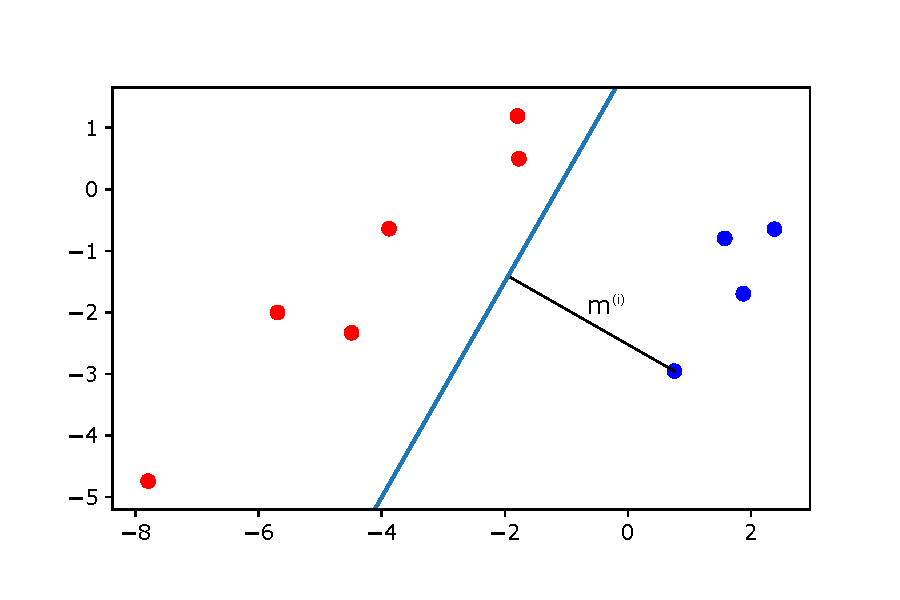
\includegraphics{distance.pdf}
\caption{Margina hiperravnine s obzirom na primjerak $(\mathbf{x}^{(i)}, y^{(i)})$}
\label{fig:mex}
\end{figure}

\par Na slici \ref{fig:mex} prikazana je udaljenost primjerka od razdvajajuće hiperravnine.
Valja uočiti kako za pozitivne oznake razreda, $y^{(i)} = 1$, vrijednost $b + \mathbf{w}^T\mathbf{x}^{(i)}$ je pozitivna.
Analogno, za $y^{(i)} = -1$ vrijednost $b + \mathbf{w}^T\mathbf{x}^{(i)}$ je negativna.
Može se zaključiti kako je vrijednost margine za svaki primjerak strogo pozitivna. 
U slučaju hiperravnine koja ne razdvaja podatke to svojstvo ne vrijedi.

\par Osim svojstva pozitivnosti, za marginu je zanimljivo i svojstvo otpornosti na skaliranje. 
Neka je hiperravnina \hiperravnina{} skalirana nekim faktorom $k$. Za marginu $m^{'(i)}$ vrijedi:
\begin{equation*}
  m^{'(i)} = \frac{y^{(i)}(kb + k\mathbf{w}^T\mathbf{x}^{(i)})}{\|k\mathbf{w}\|} =
  \frac{y^{(i)}k(b + \mathbf{w}^T\mathbf{x}^{(i)})}{k\|\mathbf{w}\|} = m^{(i)}.
\end{equation*}
Ovo svojstvo omogućuje da duljina vektora težina bude proizvoljna što će se pokazati veoma korisnim kod
postavljanja optimizacijskog problema.

\par Nakon definiranja margine hiperravnine za pojedini primjerak, potrebno je definirati 
i marginu hiperravnine uzimajući u obzir cijeli skup podataka za učenje. 
\textbf{Margina hiperravnine} u odnosu na skup podataka za učenje 
je margina onog primjerka koji je najbliži hiperravnini tj.
$$M=\min_{i}m^{(i)}.$$

\section{Optimalna razdvajajuća hiperravnina} \label{opthiper}
Nakon definicije margine, sljedeći cilj je pronaći razdvajajuću hiperravninu koja najbolje razdvaja podatke.
Uzimajući u obzir činjenicu da veća udaljenost primjerka od hiperravnine pruža veću sigurnost za ispravnu
klasifikaciju, intuitivno se može zaključiti kako će optimalna razdvajajuća hiperravnina biti ona koja
maksimizira marginu hiperravnine s obzirom na skup primjeraka za učenje. 
\textbf{Optimalna razdvajajuća hiperravnina} zadana je sljedećim optimizacijskim problemom:

\begin{equation}
\begin{aligned}
& \underset{\mathbf{w}, b}{\text{max}}
& & M \\
& \text{s obzirom na}
& & m^{(i)} \geq M, \; i = 1, \ldots, N
\end{aligned}
\end{equation}

\par Ograničenje $m^{(i)} \geq M$ zahtjeva da svi primjerci iz skupa za učenje budu udaljeni za minimalno $M$
od razdvajajuće hiperravnine. 
No, izraz \ref{eq:marg} nije konveksan stoga se redefinira na sljedeći način:
\begin{equation*}
  y^{(i)}(\mathbf{w}^T\mathbf{x}^{(i)} + b) \geq M\|\mathbf{w}\|, \; i = 1, \ldots, N.
\end{equation*}

Nadalje, budući da duljina vektora težina ne utječe na marginu i klasifikaciju, moguće je proizvoljno odabrati
njegovu duljinu.
Za $\|\mathbf{w}\|=\frac{1}{M}$ cilj optimizacije se svodi na pronalazak maksimuma funkcije 
$f^*(\mathbf{w}) = \frac{1}{\|\mathbf{w}\|}$. Znajući kako se maksimizacija ove funkcije može svesti na 
minimizaciju kvadrata norme, može se pisati:

\begin{equation}
\begin{aligned}
& \underset{\mathbf{w}, b}{\text{min}}
& & \frac{1}{2}\|\mathbf{w}\|^2 \\
& \text{s obzirom na}
& & y^{(i)}(\mathbf{w}^T\mathbf{x}^{(i)} + b) \geq 1, \; i = 1, \ldots, N.
\end{aligned}
\end{equation}

\par Koristeći nekoliko različitih transformacija, problem je redefiniran na jednostavniji način.
Budući da je dobivena konveksna kvadratna funkcija cilja uz linearne uvjete ovaj problem je rješiv
metodama kvadratnog programiranja. Kasnije će se u radu ovaj optimizacijski problem dodatno transformirati
kako bi se iskoristili algoritmi koji rješavaju problem efikasnije od općenitih programskih paketa koji
koji se koriste za rješavanje ovakvih optimizacijskih problema. 

\section{Regularizacija} \label{reg}
U dosadašnjem radu klasificiralo se linearno razdvojive podatke. 
Međutim, podaci najčešće nisu linearno razdvojivi ili optimalna razdvajajuća hiperravnina nije najbolji
klasifikator budući da nije otporna na stršeće vrijednosti.
Slučaj kada stršeća vrijednost utječe na izbor hiperravnine prikazan je na slici \ref{fig:outlier}.
Vidljivo je kako hiperravnina nacrtana plavom bojom dobro razdvaja podatke osim stršeće vrijednosti 
označene točkom $T$. Druga hiperravnina označena crnom bojom, iako je razdvajajuća, nije 
najsretniji izbor za klasifikaciju.

\begin{figure}
\centering
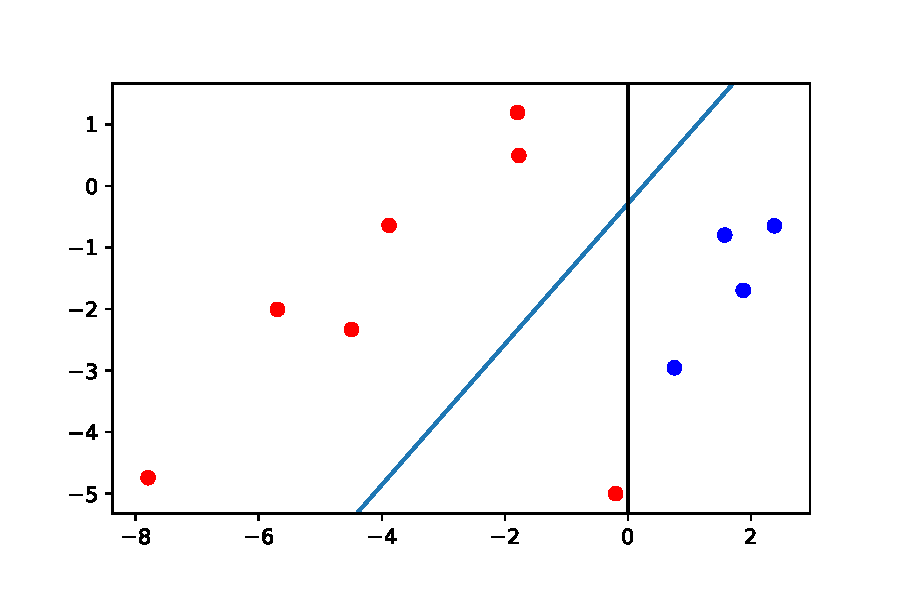
\includegraphics{outlier.pdf}
\caption{Utjecaj stršeće vrijednosti na odabir hiperravnine}
\label{fig:outlier}
\end{figure}

\par Optimizacijski problem je napisan tako da bira razdvajajuću hiperravninu u bilo kojem slučaju, čak i kada
ona nije dobar izbor. Kao rješenje ovog problema uvodi se metoda regularizacije.
\textbf{Regularizacija} je metoda kojom se sprječava pretreniranost modela koristeći funkciju kazne.
Iako je hiperravnina nacrtana crnom bojom na slici \ref{fig:outlier} dobro prilagođena danim primjercima,
kod klasificiranja novih primjerka neće dati dobre rezultate kao hiperravnina označena plavom bojom.
Ovime se kažnjavaju modeli koji pretjerano slijede sve primjerke, ne vodeći računa o generalnoj strukturi 
podataka.

\par Valja navesti dvije najosnovnije funkcije kazne koje se koriste za regularizaciju SVM modela.
Funkcija kazne kod L1-SVM modela zadana je izrazom $\text{max}(1 - y^{(i)}\mathbf{w}^T\mathbf{x^{(i)}}, 0)$, a
kod L2-SVM funkcija kazne je zadana izrazom $\text{max}(1 - y^{(i)}\mathbf{w}^T\mathbf{x^{(i)}}, 0)^2$.
U nastavku će se koristiti L1-SVM.

\par Nakon uvođenja regularizacije, optimizacijski problem može se redefinirati na sljedeći način:
\begin{equation}
\begin{aligned}
& \underset{\mathbf{w}, b}{\text{min}}
& & \frac{1}{2}\|\mathbf{w}\|^2 + C\sum_{i=1}^{N} \xi_i\\
& \text{s obzirom na}
& & y^{(i)}(\mathbf{w}^T\mathbf{x}^{(i)} + b) \geq 1 - \xi_i, \; i = 1, \ldots, N \\
&&& \xi_i \geq 0, \; i = 1, \ldots, N.
\end{aligned}
\label{eq:opt}
\end{equation}

Valja obratiti pažnju na regularizacijski parametar $C$ čiji iznos izražava spremnost na pogrešnu klasifikaciju
primjerka iz skupa za učenje.
Za velike iznose parametra $C$, optimizacija će inzistirati na ispravnoj klasifikaciji primjeraka iz skupa
za učenje, makar pod cijenu pretreniranosti. Za manje iznose, optimizacija će pogrešno klasificirati 
neke od primjeraka iz skupa za učenje kako bi se pronašla hiperravnina koja dobro opisuje generalnu strukturu
podataka.

\section{Primarni i dualni optimizacijski problem}  \label{sec:primdual}
Nakon što je optimizacijski problem postavljen, vrijedi ga pokušati i riješiti.
Postupak koji će se koristiti u rješavanju ovog problema je metoda Lagrangeovih multiplikatora.
Neka je zadan \textbf{primarni} optimizacijski problem oblika:
\begin{equation}
\begin{aligned}
& \underset{x}{\text{min}}
& & f(x)\\
& \text{s obzirom na}
& & g_i(x) \leq 0, \; i = 1, \ldots, m \\
&&& h_i(x) = 0, \; i = 1, \ldots, n.
\end{aligned}
\label{eq:lf}
\end{equation}

Za dani optimizacijski problem, može se postaviti Lagrangeova funkcija oblika:
\begin{equation}
\mathcal{L}(x, \alpha, \beta) = f(x) + \sum_{i=1}^{m}\alpha_ig_i(x) + \sum_{i=1}^{n}\beta_ih_i(x)
\end{equation}

gdje su $\alpha_i$ i $\beta_i$ Lagrangeovi multiplikatori.
Budući da se traži ekstrem funkcije, Lagrangeova funkcija se parcijalno derivira po varijablama $x, \alpha$
i $\beta$ te se parcijalne derivacije izjednače s nulom. 

\par Nakon definiranja Lagrangeove funkcije, valja definirati i još jednu vrijednost:
\begin{equation}
\begin{aligned}
& \theta_\mathcal{P}(x) = \underset{\alpha, \beta, \alpha_i \geq 0}{\text{max}}
& & \mathcal{L}(x, \alpha, \beta).\\
\end{aligned}
\end{equation}

Može se pokazati kako je iznos $\theta_\mathcal{P}(x)$ jednak vrijednosti funkcije $f(x)$ u slučaju kada su svi uvjeti
zadovoljeni. 
U slučaju da neki od uvjeta nisu zadovoljeni, $\theta_\mathcal{P}(x)$ iznosi nula.
Primjerice neka je $g_i(x) > 0$.
Tada se može izabrati $\alpha_i$ za koji desna strana jednadžbe \ref{eq:lf} iznosi $\infty$.
Analogno vrijedi i za $h_i(x) \neq 0$. 
\par Minimizacijom vrijednosti $\theta_\mathcal{P}(x)$ dobije se problem jednak primarnom.
Vrijednost primarnog problema dana je izrazom:
\begin{equation}
\begin{aligned}
& p = \underset{x}{\text{min}}
& & \theta_\mathcal{P}(x).\\
\end{aligned}
\end{equation}

\par Za pronalazak $\theta_\mathcal{P}(x)$ interesantan je bio maksimum Lagrangeove funkcije u odnosu na 
parametre $\alpha$ i $\beta$.
Umjesto toga, problem se može modificirati da umjesto traženja maksimuma u odnosu na parametre $\alpha$ i $\beta$,
traži se minimum u odnosu na $x$. 
\textbf{Dualni} problem definira se na sljedeći način:
\begin{equation}
\underset{\alpha, \beta, \alpha_i \geq 0}{\text{max}} \theta_\mathcal{D}(x) = 
\underset{\alpha, \beta, \alpha_i \geq 0}{\text{max}} \underset{x}{\text{min}} \; \mathcal{L}(x, \alpha, \beta).
\end{equation}

\par Valja primijetiti kako je dualni problem jednak primarnom, uz zamjenu poretka funkcije $min$ i funkcije $max$.
Vrijednost $\theta_\mathcal{D}(x)$ je dana izrazom:

\begin{equation}
\begin{aligned}
& d = \underset{\alpha, \beta, \alpha_i \geq 0}{\text{max}}
& & \theta_\mathcal{D}(x).\\
\end{aligned}
\end{equation}

Uzimajući u obzir odnos između funkcija $max$ i $min$ jasno je da vrijedi relacija $d \leq p$.
No, posebno su interesantni slučajevi gdje su vrijednosti primarnog i dualnog problema jednake.

\par Kako bi vrijednost primarnog i dualnog problema bila jednaka, potrebno je postaviti neka ograničenja
na funkcije $f, g_i$ i $h_i$. Neka je $f$ konveksna funkcija. Nadalje, neka su $g_i$ konveksne funkcije 
i neka za svaku od njih vrijedi $g_i(x) < 0$. 
Također, neka je $h_i$ linearna funkcija. 
Ako su ti uvjeti zadovoljeni, tada postoje $\alpha, \beta$ i $x$ za koje vrijedi sljedeća jednakost: 
\begin{equation}
  p = d = \mathcal{L}(x, \alpha, \beta).
\end{equation}

Osim gornje jednakosti, za parametre vrijede i Karush-Kuhn-Tucker (KKT) uvjeti:
\begin{equation}
  \frac{\partial \mathcal{L}(x, \alpha, \beta)}{\partial x_i} = 0, \; i = 1, \ldots, p
\end{equation}
\begin{equation}
  \frac{\partial \mathcal{L}(x, \alpha, \beta)}{\partial \beta_i} = 0, \; i = 1, \ldots, n
\end{equation}
\begin{equation}
  \alpha_ig_i(x) = 0, \; i = 1, \ldots, m
  \label{eq:inter}
\end{equation}
\begin{equation}
  g_i(x) \leq 0, \; i = 1, \ldots, m
\end{equation}
\begin{equation}
  \alpha_i \geq 0, \; i = 1, \ldots, m
\end{equation}

Valja napomenuti kako se kod optimizacije stroja s potpornim vektorima u pravilu koristi dualni problem.
Također, za SVM interesantan je uvjet zadan jednakošću \ref{eq:inter}. U pravilu $\alpha_i \neq 0$ iz čega
slijedi $g_i(x) = 0$. Taj uvjet je ključan za pronalazak potpornih vektora.

\section{Optimizacija stroja s potpornim vektorima} \label{sec:svmopt}
Primjenjujući prethodno potpoglavlje na optimizacijski problem 
iz potpoglavlja \ref{eq:opt}, primarna Lagrangeova funkcija može se zapisati
na sljedeći način:
\begin{equation} \label{eq:svmprim}
  \mathcal{L}(\mathbf{w}, b, \xi,\alpha, \mu) = \frac{1}{2}\|\mathbf{w}\|^2 + C\sum_{i=1}^{N} \xi_i
  - \sum_{i=1}^{N} \alpha_i(y^{(i)}(\mathbf{w}^T\mathbf{x^{(i)}} + b) - (1 - \xi_i))
  - \sum_{i=1}^{N} \mu_i\xi_i.
\end{equation}

Vidljivo je kako je ograničenje $y^{(i)}(\mathbf{w}^T\mathbf{x}^{(i)} + b) \geq 1 - \xi_i$ zapisano
kao:
\begin{equation*}
  g_i(\mathbf{w}, b) = - (y^{(i)}(\mathbf{w}^T\mathbf{x^{(i)}} + b) - (1 - \xi_i)) \leq 0.
\end{equation*}

Gore navedeno ograničenje ima zanimljivo svojstvo. 
U slučaju da vrijedi $g_i(\mathbf{w}, b) = 0$ za neki primjerak $(x^{(i)}, y^{(i)})$ tada
se taj primjerak naziva \textbf{potpornim vektorom}. Može se pretpostaviti kako je potpornih vektora 
relativno malo u odnosu na cijeli skup primjeraka za učenje. Vodeći se tom pretpostavkom te uvjetom \ref{eq:inter}
može se zaključiti kako samo za potporne vektore vrijedi $\alpha_i \neq 0$ dok za ostale primjerke vrijedi 
$\alpha_i = 0$.

\begin{figure}
\centering
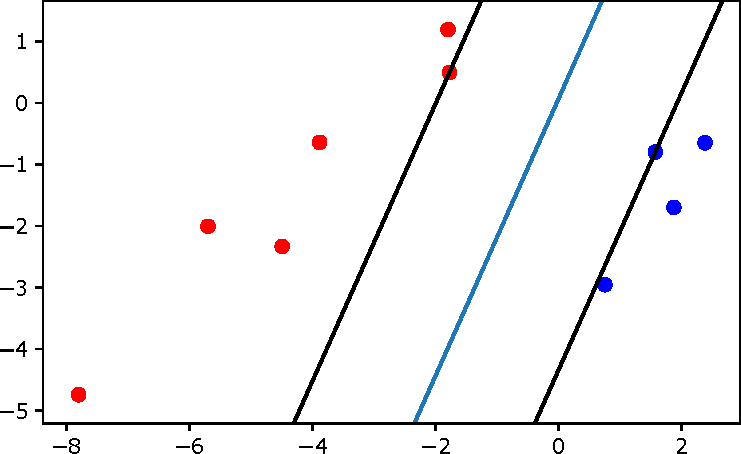
\includegraphics{support.pdf}
\caption{Maksimalna razdvajajuća hiperravnina te pravci na kojima leže potporni vektori}
\label{fig:support}
\end{figure}

Na slici \ref{fig:support} prikazana je maksimalna razdvajajuća hiperravnina te pravci paralelni s istom 
na kojima leže potporni vektori. Valja primijetiti kako su pravci jednako udaljeni od hiperravnine za
iznos $M$.

\par Primarni problem dan izrazom \ref{eq:svmprim} može se derivirati po $\mathbf{w}, b$ i $\xi_i$
te izjednačiti s nulom:
\begin{equation}
  \mathbf{w} = \sum_{i=1}^{N} \alpha_iy^{(i)}x^{(i)}
\end{equation}
\begin{equation} \label{eq:dualcomp}
  0 = \sum_{i=1}^{N} \alpha_iy^{(i)}
\end{equation} 
\begin{equation}
  \alpha_i = C - \mu_i, \forall i.
\end{equation}

Ubacivanjem gornjih izraza u \ref{eq:svmprim}, dolazi se do dualne Lagrangeove funkcije:
\begin{equation} \label{eq:svmdual}
  \mathcal{L}(\alpha) = \sum_{i=1}^{N} \alpha_i - 
  \frac{1}{2}\sum_{i=1}^{N}\sum_{j=1}^{N} \alpha_i\alpha_jy^{(i)}y^{(j)}x^{(i)T}x^{(j)}.
\end{equation}

Uz ograničenje \ref{eq:dualcomp} te ograničenje $0 \leq \alpha_i \leq C$ dualni problem može se zapisati
na sljedeći način:
\begin{equation} \label{eq:dualprob}
\begin{aligned}
& \underset{\alpha}{\text{max}}
& & \sum_{i=1}^{N} \alpha_i - 
  \frac{1}{2}\sum_{i=1}^{N}\sum_{j=1}^{N} \alpha_i\alpha_jy^{(i)}y^{(j)}x^{(i)T}x^{(j)}\\
& \text{s obzirom na}
& & 0 \leq \alpha_i \leq C, \; i = 1, \ldots, N \\
&&& \sum_{i=1}^{N} \alpha_iy^{(i)} = 0.
\end{aligned}
\end{equation}

Ako se pogleda uvjet \ref{eq:dualcomp} može se zaključiti kako samo potporni vektori utječu na
odabir hiperravnine. U slučaju linearno nerazdvojivih podataka za potporne vektore koji se nalaze
na margini, Lagrangeov multiplikator iznosi $0 < \alpha_i < C$. U slučaju da se potporni vektor ne
nalazi na margini, vrijednost pripadajućeg multiplikatora iznosi $C$.

\section{Jezgreni trikovi} \label{jezgra}
Dosad je optimizacija stroja s potpornim vektorima mogla pronaći razdvajajuću hiperravninu jedino u
slučaju linearno razdvojivih podataka. 
Želja je izgraditi klasifikator koji će moći ispravno klasificirati podatke koji su nisu linearno 
razdvojivi.

\par Kod metoda poput logističke regresije svaki vektor značajki može se, koristeći mapiranje značajki,
preslikati u neki drugi vektor značajki.
Neka je $\mathbf{x}=(x_1, \ldots, x_p)$ vektor značajki. 
Radi jednostavnosti neka postoji samo jedna značajka tj. $\mathbf{x} = (x_1)$.
Neka funkcija $\phi$ vrši polinomijalno mapiranje značajki do trećeg stupnja tj. 
$\phi(x) = (x, x^2, x^3)$. 
Tada vektor značajki $\mathbf{x}$ može se preslikati u 
$\mathbf{x}^{'} = \phi(x_1) = (x_1, x_1^2, x_1^3)$.
Ova ideja može se iskoristiti i kod stroja s potpornim vektorima.
Svaku pojavu vektora značajki $\mathbf{x}$ moguće je zamijeniti funkcijom $\phi(\mathbf{x})$.

\par Valja se na trenutak vratiti na dualnu Lagrangeovu funkciju zadanu jednakošću \ref{eq:svmdual}.
Može se primijetiti kako dio funkcije zadan izrazom $x^{(i)T}x^{(j)}$ je zapravo skalarni umnožak vektora
značajki dvaju primjera. Nadalje će se pisati $\langle x^{(i)},x^{(j)} \rangle$. 
Vektore značajki moguće je preslikati u neke nove vektore značajki koristeći funkciju $\phi$. 
Vrijedi:
\begin{equation*}
  \mathcal{L}(\alpha) = \sum_{i=1}^{N} \alpha_i - 
  \frac{1}{2}\sum_{i=1}^{N}\sum_{j=1}^{N} \alpha_i\alpha_jy^{(i)}y^{(j)}
  \langle \phi(x^{(i)}), \phi(x^{(j)}) \rangle.
\end{equation*}

Primjerak $(x^{(i)}, y^{(i)})$ tada se klasificira na sljedeći način:
\begin{equation*}
  \hat{y} = sgn(\sum_{i=1}^{N} \alpha_iy^{(i)}\langle \phi(x), \phi(x^{(i)}) \rangle
  + b).
\end{equation*}

Vidljivo je kako i dualni problem i funkcija klasifikacije koriste funkciju oblika
$\langle \phi(x), \phi(x') \rangle$, a ne $\phi(x)$. 
Može se definirati \textbf{jezgrena funkcija} oblika:
\begin{equation} \label{eq:trik}
  K(x, x') = \langle \phi(x), \phi(x') \rangle.
\end{equation}

Zamjena skalarnog umnoška vektora $x$ i $x'$ s jezgrenom funkcijom $K(x, x')$ naziva se
\textbf{jezgreni trik}. 
Najčešće korištene jezgrene funkcije su radijalna bazna funkcija (RBF), polinomijalna i 
sigmoidalna jezgrena funkcija. 

\begin{figure}
\centering
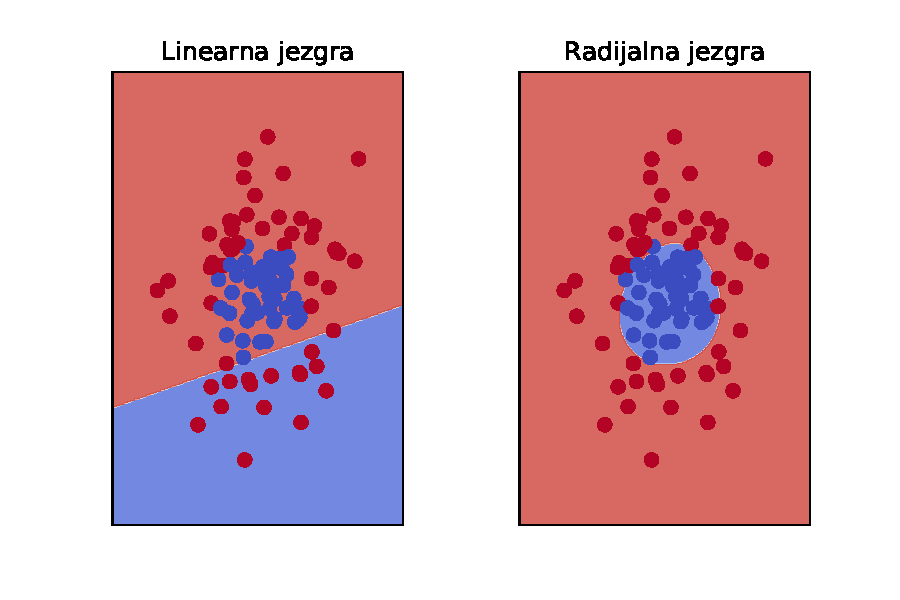
\includegraphics{kernel.pdf}
\caption{Klasifikacija podataka bez jezgrenog trika i s radijalim jezgrenim trikom}
\label{fig:kernel}
\end{figure}

Na slici \ref{fig:kernel} prikazana je kalsifikacija podataka bez korištenja jezgrenog trika i s 
korištenjem radijalne bazne funkcije. Jasno je kako linarni model nije dovoljno moćan klasificirati
ovaj skup linearno nerazdvojivih podataka. 
Radijalni bazni model je puno uspješniji u tom zadatku.

Radijalna bazna funkcija korištena u prethodnom primjeru ima oblik:
\begin{equation*}
  K(\mathbf{x}, \mathbf{x}') = \text{exp}(- \frac{\|\mathbf{x} - \mathbf{x}'\|}{2\sigma^2})
\end{equation*}
gdje je $\sigma$ parametar funkcije. Sigmoidalna jezgrena funkcija dana je oblikom:
\begin{equation*}
  K(\mathbf{x}, \mathbf{x}') = \text{tanh}(\gamma\mathbf{x}^T\mathbf{x}' + r)
\end{equation*}
gdje su $\gamma$ i $r$ parametri funkcije.
Polinomijalna jezgrena funkcija zadana je jednadžbom:
\begin{equation*}
  K(\mathbf{x}, \mathbf{x}') = (\mathbf{x}^T\mathbf{x}' + k)^d,
\end{equation*}
gdje je $k$ proizvoljna konstanta, a $d$ stupanj polinoma.
Na primjer, zadan je vektor značajki $\mathbf{x} = (x_1, x_2)$. 
Neka je $k=1$ i $d=2$. Jezgrena funkcija tada iznosi:
\begin{equation*}
  K(\mathbf{x}, \mathbf{x}') = (\mathbf{x}^T\mathbf{x}' + 1)^2 =
  1 + 2x_1x'_1 + 2x_2x'_2 + (x_1x'_1)^2 + (x_2x'_2)^2 + 2x_1x'_1x_2x'_2.
\end{equation*}
Vidljivo je kako smo vektor značajki s dva svojstva mapirali na vektor značajki sa šest svojstava.
Općenito, polinomijalna jezgrena funkcija $d$-tog reda, preslika vektor značajki duljine $p$ u 
vektor značajki duljine $\binom{n + d}{d}$.
Iz povećanja dimenzionalnosti proizlazi i jedan od problema jezgrenih funkcija.
Naime, neka su podaci linearno razdvojivi u slučaju prostora koji sadrži interakcijsku značajku
$x_1x'_1$. Tada je moguće, koristeći gore navedenu polinomijalnu funkciju drugog stupnja, pronaći
razdvajajuću hiperravninu. No, uz pronalazak težine za tu značajku optimizacija traži i težine za ostalih 
pet značajki. Ovaj problem s povećanjem reda jezgrene funkcije postaje sve izraženiji, pogotovo ako je
inicijalni prostor svih primjeraka velike dimenzije.

\section{Višerazredna klasifikacija} \label{sec:multiclass}
Stroj s potpornim vektorima je binarni klasifikator te kao takav nije u mogućnosti klasificirati
primjerke u više od dva razreda.
To ograničenje je intuitivno budući da hiperravnina dijeli prostor u dva potprostora.
Za rješenje ovog problema nude se dvije često korištene metode višerazredne klasifikacije.

\par Prva metoda višerazredne klasifikacije je metoda "jedan-naspram-ostalih" (engl. \textit{one-vs-all}).
Koristeći ovu metodu gradi se sustav klasifikatora.
Ako je zadano $N$ različitih razreda, sustav će biti izgrađen od $N-1$ klasifikatora.
Ovom metodom problem se razbija u više binarnih klasifikacija.
Svaki stroj vrši klasifikaciju za pojedini razred. Vrijednost $1$ označava pripadnost tom razredu dok
vrijednost $-1$ kaže kako primjerak ne pripada razredu.
U slučaju da svih $N-1$ klasifikatora daju negativan izlaz, tada primjerak pripada zadnjem,
$N$-tom razredu. Problem kod ove metode je mogućnost pozitivnog izlaza za više klasifikatora.
Tada sustav nije u mogućnosti odrediti razred kojemu primjerak pripada.

\par Druga metoda višerazredne klasifikacije je metoda "jedan-naspram-jedan" (engl. \textit{one-vs-one}).
Kod ove metode također se gradi sustav klasifikatora, ali kod ove metoda jedan klasifikator vrši usporedbu
između dvaju razreda.
Ukupan broj izgrađenih klasifikatora iznosi $\frac{N(N - 1)}{2}$.
Očito je kako je ova metoda vremenski složenija od "jedan-naspram-ostalih" metode. 
No, ova metoda je robusnija u slučaju linearno nerazdvojivih podataka te je robusnija na gore navedeni 
problem koji se javlja kod "jedan-naspram-ostalih" metode.
Sustav radi na principu glasanja. 
Prilikom klasifikacije, svaki klasifikator daje glas nekom od relevantnih razreda. 
Primjerak pripada nekom razredu u slučaju da je taj razred dobio najviše glasova.

\section{Primjena SVM-a kod regresijskih problema} \label{sec:svr}
Stroj s potpornim vektorima je primarno binarni klasifikator. 
No, Drucker je 1997. godine predložio proširenje stroja s potpornim vektorima na 
probleme regresije \cite{Drucker97supportvector}.

\par Neka je zadan linearan model oblika:
\begin{equation}
  f(\mathbf{x}) = \mathbf{w}^T\mathbf{x} + b. 
\end{equation}

Moguće je zapisati funkciju optimizacije na sljedeći način:
\begin{equation}
  f(\mathbf{w}, b) = \frac{1}{2}\|\mathbf{w}\|^2 + 
  C\sum_{i=1}^{N}L(y^{(i)} - f(\mathbf{x}^{(i)}))
\end{equation}
gdje je $L$ funkcija kazne, a $C$ regularizacijski parametar. 
Funkciju kazne $L$ moguće je izabrati na nekoliko načina. 
Neka je $d$ razlika između dane vrijednosti $y^{(i)}$ i vrijednosti izračunate modelom $f(\mathbf{x}^{(i)})$
za neki primjerak $(\mathbf{x}^{(i)}, y^{(i)})$. 
U slučaju da je greška manja od neke proizvoljne vrijednosti $\epsilon$ tada taj primjerak ne pridonosi
ukupnoj grešci. 
U slučaju pogreške veće od $\epsilon$, primjerak pridonosi ukupnoj grešci s $|d| - \epsilon$.
Uspoređujući ovu funkciju kazne s načinom rada klasifikatora može se ustvrditi sličnost.
Za primjerke koji su jako udaljeni od hiperravnine, klasifikator je veoma siguran da su oni ispravno 
klasificirani te ne utječu na optimizaciju, za razliku od potpornih vektora. 
Kod regresije, primjerci koji su relativno blizu svojoj očekivanoj vrijednosti ne pridonose povećanju
iznosa kazne. Može se pisati:

\begin{equation}
  L(d) = 
  \begin{cases}
    0 & \quad |d| < \epsilon\\
    |d| - \epsilon & \quad \text{inače}.\\
  \end{cases}
\end{equation}

Koristeći gore navedene podatke, može se napisati optimizacijska funkcija:
\begin{equation*}
  f(\alpha, \alpha') = \epsilon \sum_{i=1}^{N} (\alpha'_i + \alpha_i) - 
  \sum_{i=1}^{N} y^{(i)}(\alpha'_i - \alpha_i) + \frac{1}{2}\sum_{i=1}^{N}\sum_{j=1}^{N}
(\alpha'_i - \alpha_i)(\alpha'_j - \alpha_j)\langle x^{(i)},x^{(j)} \rangle
\end{equation*}

i pripadajući optimizacijski problem:

\begin{equation}
\begin{aligned}
& \underset{\alpha, \alpha'}{\text{min}}
& & f(\alpha, \alpha')\\
& \text{s obzirom na}
& & \alpha_i \geq 0, \\
&&& \sum_{i=1}^{N} (\alpha'_i - \alpha_i) = 0,\\
&&& \alpha'_i \leq C,\\
&&& \alpha_i\alpha'_i = 0.
\end{aligned}
\end{equation}

U ovom slučaju primjerci za koje vrijedi $\alpha'_i - \alpha_i \neq 0$ nazivaju se potpornim vektorima.
Metode koje se koriste za optimizaciju klasifikacijskog stroja mogu se koristiti i za optimizaciju
regresijskog stroja.

\chapter{Analiza sentimenta} \label{sentiment}
Ovo poglavlje je posvećeno problemu analize sentimenta.
Potpoglavlje \ref{def} iznosi definiciju problema analize sentimenta.
U potpoglavlju \ref{samisljenje} pojašnjeni su tipovi mišljenja u analizi sentimenta.
Potpoglavlje \ref{sarazine} daje pregled razina u analizi sentimenta, a potpoglavlje \ref{sadoc} 
fokusira se na razinu dokumenta.
Zadnje potpoglavlje \ref{saprob} daje pregled problema s kojima se susreće prilikom analize sentimenta.

\section{Definicija} \label{def}
Analiza sentimenta (engl. \textit{Sentiment Analysis}) je područje posvećeno 
prikupljanju, obradi i analizi subjektivnih informacija, posebice stavova.
Subjektivne informacije podrazumijevaju kratkoročna stanja poput emocija i raspoloženja,
dugoročna stanja poput stavova pa čak i psihičkih osobina.
S druge strane, objektivne rečenice izriču činjenice. 
Primjerice objektivna rečenica \textit{"Danas je sunčano."} izražava činjenicu te se iz nje ne mogu 
iščitati emocije, stavovi i slično. 
Rečenica poput \textit{"Volim sunčan dan."} govori kako izvor mišljenja ima pozitivan stav prema danima koji
sunčani te je stoga ova rečenica subjektivna.
Moguće je da subjektivna rečenica ne izriče stav. 
Rečenica \textit{"Mislim da će sutra biti sunčan dan."} ne predstavlja nikakvu činjenicu, već subjektivni dojam,
no ne izriče nikakav sentiment. 

\par Najčešće promatrana stanja su stavovi pojedinca koji predstavljaju enormni izvor korisnih 
informacija za zainteresirani subjekt.
Koristeći ove informacije, političari mogu osvajati i gubiti izbore, poduzeća plasirati
svoje usluge i proizvode, a potrošači informirati se o istima.
Uporabom metoda obrade prirodnog teksta i metoda strojnog učenja, cilj je automatizirati
obradu i analizu subjektivnih informacija.
Upravo subjektivnost čini ovo područje teškim i istovremeno zanimljivim.

\par Problem analize sentimenta može se zadati i na formalniji način.
Neka je dana uređena petorka $(o, k, i, s, v)$ kojom se može definirati sentiment 
\cite{Liu:2012:SAO:3019323}.
Varijabla $o$ predstavlja promatrani objekt. 
Primjerice, ako se analizira kvaliteta mobilnih uređaja, promatrani objekt upravo 
bi bili mobilni uređaji. Varijablom $k$ dana je karakteristika promatranog objekta. 
U slučaju mobilnih uređaja to bi mogla biti kamera, ekran, zvuk, itd.
Ako se analizira uređaj u cjelini, tada ova varijabla može biti zanemarena.
Varijabla $i$ predstavlja izvor mišljenja, najčešće korisnika neke usluge ili proizvoda.
Ključni dio problema, sentiment, dan je varijablom $s$. 
Sentiment predstavlja mišljenje korisnika $i$ o nekoj karakteristici $k$ proizvoda $o$.
Mišljenja, stavovi i emocije mijenjaju se s vremenom pa je važno uključiti i vrijeme u sam
problem. 
Vrijeme je predstavljeno varijablom $v$.

\par Evo i jednog primjera korisničke recenzije operacijskog sutava\footnote{Napomena: 
Iako nije dano ime operacijskog sustava, čitatelj može s jednostavnošću
zaključiti o kojem se operacijskom sustavu radi}: \\
{\it
Užasan operacijski sustav. 
Osim osnovnih alata, upakiran je i s gomilu programa koji samo usporavaju rad sustava.
Nadam se da korisnici nisu ljubitelji privatnosti jer ju s ovim operacijskim sustavom
sigurno neće imati. 
Jedina pozitivna opcija je uvođenje radnih sati tako da me sustav rjeđe maltretira s 
ponovnim pokretanjem.
Savjet: potražite alternativu.
} Marko, 2016.
\par Nakon čitanja korisničke recenzije, jasno je kako se ovdje radi o negativnoj recenziji
proizvoda.
Prva rečenica recenzije je najbitnija za određivanje sentimenta prema cijelom proizvodu.
Izvor mišljenja, korisnik Marko, ocjenjuje cijeli sustav \textit{užasnim}.
Izbor pridjeva, u ovom slučaju \textit{užasan}, sigurno utječe na intenzitet sentimenta. 
Kad bi se umjesto navedenog pridjeva našao pridjev \textit{loš} i dalje bi izjava bila
klasificirana kao negativna, no s puno manjim intenzitetom u odnosu na izjavu koja sadrži pridjev 
\textit{užasan}.
Valja napomenuti kako kontekst također utječe na pozitivnost sentimenta.
U ovom primjeru, riječ \textit{užasan} je nositelj negativnog sentimenta. 
No, u izrazu \textit{užasno pametan} riječ \textit{užasno} ističe poztivinu karakteristiku objekta.
Nakon prve rečenice, slijede dvije rečenice negativnog sentimenta usmjerene na pojedine karakteristike
sustava. Četvrta rečenica navodi jednu pozitivnu karakteristiku sustava.
U slučaju analize sentimenta na razini cijele recenzije ova rečenica uvodi šum te predstavlja jedan od
problema u analizi sentimenta. 
Iz zadnje rečenice, iako svakako manjeg intenziteta od ostalih, također se može iščitati negativan 
stav prema proizvodu. Valja napomenuti kako je ova recenzija napisana 2016. godine te upravo godina 
predstavlja vremensku komponentu problema. Moguće je da se s vremenom stav korisnika promijeni.
Tada ova recenzija više neće biti aktualna. Ukupno se može iščitati četiri sentimenta: 
\begin{center}
(Operacijski sustav, "općenito", Marko, negativan, 2016.)\\
(Operacijski sustav, programski paket, Marko, negativan, 2016.)\\
(Operacijski sustav, razina privatnosti, Marko, negativan, 2016.)\\
(Operacijski sustav, vrijeme osvježavanja sustava, Marko, pozitivan, 2016.) \\
\end{center}

\section{Tipovi mišljenja} \label{samisljenje}
Postoji nekoliko podjela mišljenja. 
Najčešće korišten tip mišljenja u analizi sentimenta je regularno mišljenje.
Uz regularno mišljenje, izdvaja se i komparativno mišljenje.
Alternativna podjela je podjela mišljenja na implicitno i eksplicitno mišljenje.

\begin{enumerate}
  \item \textbf{Regularno mišljenje} je najčešći tip mišljenja te unutar njega postoje dva podtipa mišljenja.
  Izravno mišljenje je mišljenje u kojem korisnik jasno izražava svoje mišljenje. 
  Rečenica \textit{Volim kolače.} je primjer izravnog mišljenja.
  S druge strane, neizravno mišljenje karakterizira neizravno iskazivanje mišljenja o objektu.
  Najčešće izvor mišljenja iskazuje osjećaj prouzročen utjecajem objekta na njega.
  Primjer neizravnog mišljenja je rečenica \textit{"Konzumiranje kolača povećava moje zadovoljstvo."}.
  U istraživanju, naglasak je stavljen na izravno mišljenje budući da ga je lakše uočiti i analizirati.

  \item \textbf{Komparativno mišljenje} iskazuje odnos između dva objekta ili karakteristike.
  Često se kod komparativnog mišljenja koristi stupnjevanje pridjeva kako bi se definirao 
  odnos. 
  Rečenica \textit{"Iako volim voćne kolače, draži su mi čokoladni."} je primjer komparativnog mišljenja.
  U ovoj rečenici iskazan je pozitivan sentiment prema voćnim i čokoladnim kolačima, no očito je
  kako su mišljenja različitih intenziteta.

  \item \textbf{Eksplicitno mišljenje} je tip mišljenja iz kojeg je direktno moguće iščitati
  regularno ili komparativno mišljenje. Rečenica \textit{"Volim kolače."} primjer je eksplicitnog
  mišljenja.

  \item \textbf{Implicitno mišljenje} je objektivna izjava koja implicira regularno ili komparativno
  mišljenje. Ovakav tip mišljenja kroz činjenice ističe sentiment korisnika.
  Primjer implicitnog mišljenja je rečenica \textit{"Baterija na mobitelu ne traje dovoljno dugo."}.
\end{enumerate}

Može se zaključiti kako je tanka granica između ovih podjela, posebno u slučaju izravnih i neizravnih
mišljenja te eksplicitnih i implicitnih mišljenja. U pravilu fokus je na izravnim i eksplicitnim
mišljenjima budući da je detekcija i analiza lakša u odnosu na neizravna i implicitna mišljenja.

\section{Razine analize sentimenta} \label{sarazine}
Sentiment korisnika može se proučavati na više razina.
U pravilu sentiment korisnika proučava se na sljedeće tri razine:

\begin{enumerate}
  \item \textbf{Analiza na razini dokumenta}. 
  Cilj ove razine je pronaći generalni sentiment u sklopu cijelog teksta. 
  Provodi se najčešće kada zainteresirane strane ne zanima sentiment neke karakteristike proizvoda
  ili usluge već generalan stav.
  Također, pretpostavlja se da korisnik ocjenjuje samo jedan proizvod budući da iz njega nije moguće
  iščitati mišljenje o više proizvoda.
  Primjer analize na razini dokumenta je analiza korisničkih recenzija filmova 
  \cite{Pang+Lee+Vaithyanathan:02a}.

  \item \textbf{Analiza na razini rečenica}.
  Cilj analize na razini rečenica je odrediti pozitivnost, neutralnost ili negativnost svake rečenice.
  Za ovu razinu analize važno je razlikovati objektivne i subjektivne rečenice 
  \cite{wiebe-bruce-o'hara:1999:ACL}.
  No, postoje iznimke kada rečenice, iako objektivne, nose sentiment.
  Primjerice, \textit{"Kapacitet baterije ovoga mobitela drastično opada već nakon dva mjeseca."}
  predstavlja objektivnu rečenicu, ali i implicitno izlaže nezadovoljstvo korisnika.

  \item \textbf{Analiza na razini karakteristika}.
  Najdetaljnija i najkompleksnija analiza sentimenta vrši se na razini karakteristika.
  Pretpostavka je da svako mišljenje sadrži sentiment i objekt te da mišljenje nije striktno vezano
  uz formu tj. uz rečenicu, paragraf, cijeli dokument \cite{Hu:2004:MSC:1014052.1014073}.
  Na primjer, rečenica \textit{"Zadovoljan sam s mobitelom marke A, no nije kao onaj marke B."}
  izražava pozitivan stav prema oba mobitela, no intenzitet sentimenta nije jednak prema oba mobitela.
  Vidljivo je kako postoji dva sentimenta i dva različita objekta što se ne može utvrditi na razini rečenice,
  a pogotovo ne na razini dokumenta.
  Rečenica \textit{"Auto je brz, ali troši previše goriva."} izražava sentiment o jednom objektu, autu, 
  ali za više njegovih karakteristika.
  Upravo je pronalazak karakteristika i objekata veoma složen problem koji čini ovu razinu još kompleksnijom
  u odnosu na razine dokumenta i rečenice. 
\end{enumerate}

Iako su sve tri razine analize sentimenta zanimljive i složene, u ovom radu fokus je stavljen na 
razinu dokumenta.

\section{Sentiment na razini dokumenta} \label{sadoc}
Analiza sentimenta na razini dokumenta najčešće je obrađivan problem u ovom području.
Cilj analize na razini dokumenta je pronaći sentiment osnovne informacijske jedinice, u ovom slučaju
cijelog dokumenta.
U pravilu ova razina se najčešće bavi sentimentom korisnika prema različitim proizvodima i uslugama.
Budući da se analizom dolazi do generalnog sentimenta, ova razina analize nije pogodna za pronalazak
sentimenta u odnosu na karakteristike proizvoda ili sentimenta za više različitih proizvoda.

\par Problem analize sentimenta na razini dokumenta može se definirati i na formalniji način. 
Cilj analize sentimenta na razini dokumenta je pronaći sentiment $s$ izvora mišljenja $i$ 
o objektu $o$ pri čemu se ne analiziraju karakteristike objekta \cite{Liu:2012:SAO:3019323}. 
Problem se predstavlja uređenom petorkom: $(\text{\_}, \text{"općenito"}, \text{\_}, s, \text{\_})$.
Pretpostavka je da su vrijeme mišljenja, izvor mišljenja te objekt znani ili nebitni za analizu.
Prilikom analize sentimenta na ovoj razini ključna je pretpostavka kako u analiziranom dokumentu
jedan izvor mišljenja izlaže stav o jednom objektu \cite{opinion.review.2010}.
U pravilu, recenzije proizvoda i usluga zadovoljavaju ovu pretpostavku.
S druge strane, transkripti političkih rasprava su primjer dokumenata koji ne zadovoljavaju pretpostavku.

\par U srži problema analize sentimenta su značajke teksta i izraza unutar njega.
Postoji nekoliko značajki koje se uzimaju u obzir prilikom analize sentimenta:

\begin{enumerate}
  \item \textbf{Subjektivne riječi i izrazi} su ključni za ispravnu klasifikaciju sentimenta.
  Riječi poput \textit{sretan}, \textit{razočaran} i \textit{odličan} uvelike određuju sentiment.
  U pravilu pridjevi i prilozi su nosioci sentimenta dok imenice i glagoli najčešće ne iskazuju sentiment.
  Čest postupak koji se koristi prilikom analize sentimenta je \textbf{označavanje} vrsta riječi.
  Primjer pridruživanja kategorija riječima su Pennove banke stabala \cite{Marcus93buildinga}.

  \item \textbf{Frekvencija izraza} nastavlja se na ideju pronalaska subjektivnih riječi.
  Osim što je važna prisutnost subjektivnih izraza, važna je i njihova učestalost.
  Dokument koji obiluje pozitivnim subjektivnim izrazima poput \textit{dobar}, \textit{sretan}, 
  itd. vjerojatno će biti klasificiran kao pozitivan.
  Uz frekvenciju izraza, često se koristi i relevantnost izraza koja daje mjeru o važnosti pojedinog
  izraza za neki dokument.

  \item \textbf{Negacija} je izdvojena kao posebna značajka budući da njena prisutnost drastično mijenja 
  sentiment. Rečenica \textit{"Ovo prijenosno računalo je dobro."} bit će klasificirana kao pozitivna.
  No, rečenica \textit{"Ovo prijenosno računalno nije dobro."} klasificirat će se kao negativna upravo zbog
  negacije \textit{nije} koja utječe na pridjev \textit{dobar} dajući mu suprotno značenje. 
\end{enumerate}

\par Za kraj ovog poglavlja, valja u nekoliko rečenica dati i kratki osvrt na klasifikacijske metode
prilikom analize sentimenta na razini dokumenta. 
U pravilu se za klasifikaciju sentimenta koriste metode nadziranog strojnog učenja.
Predstavnici navedenih metoda su naivni Bayesov klasifikator i stroj s potpornim vektorima.
U pravilu stroj s potpornim vektorima je nešto bolji u odnosu na Bayesov klasifikator, no obije metode
postižu zadovoljavajuće rezultate \cite{Pang+Lee+Vaithyanathan:02a}.
Osim klasičnog strojnog učenja, javljaju se i neke druge metode poput vrednovanja koje pridružuje ocjenu 
skupu značajki te pridruženu ocjenu koristi za klasifikaciju \cite{Dave:2003:MPG:775152.775226}.
Popularizacijom metoda dubokog učenja, istraživanja su krenula i u tom pravcu \cite{Socher-etal:2013}.
Valja napomenuti kako se osim binarne klasifikacije koja određuje je li tekst pozitivan ili negativan 
koristi i klasifikacija koja dokumentima pridaje ocjenu, najčešće od 1 do 5. 
Pritom ocjene 1 i 2 su negativne, 3 predstavlja neutralan sentiment, a 4 i 5 predstavlja pozitivan 
sentiment. 
Pokazalo se kako je regresijski stroj s potpornim vektorima bolji izbor kod ovakve formulacije problema
u odnosu na sustave SVM-a koristeći višerazrednu klasifikaciju \cite{Pang:2005:SSE:1219840.1219855}.

\section{Problemi kod analize sentimenta} \label{saprob}
Prilikom analize sentimenta često se javljaju problemi vezani uz prirodnu obradu jezika te uz same korisnike.
Za neke od njih, na žalost, još ne postoji efikasna metoda rješavanja istih.
Neki od najčešćih problema su:

\begin{enumerate}
  \item \textbf{Dvoznačnost} je jedan od velikih problema analize sentimenta često utječući na kvalitetu 
  klasifikacije.
  Primjerice rečenica \textit{"Ova kamera ubija."} predstavlja pozitivan sentiment dok rečenica
  \textit{"Droga ubija!"} implicitno izražava korisnikov negativan stav prema psihoaktivnim supstancama.

  \item Na problem dvoznačnosti naslanja se i problem \textbf{nositelja sentimenta}. Korisnik u pravilu
  koristi izjavne rečenice kako bi izrazio svoj sentiment. U rečenici \textit{"Ovaj film je dosadan."}
  riječ \textit{dosadan} je nositelj sentimenta.
  S druge strane, u rečenici \textit{"Ovaj film je dosadan?"} riječ više ne nosi nikakav sentiment budući
  da se više ne radi o izjavnoj, već o upitnoj rečenici.

  \item Zanimljiv problem na koji se nailazi prilikom analize sentimenta je \textbf{sarkazam}.
  Sarkazam se najčešće ne pojavljuje u recenzijama proizvoda i usluga, no čest je u raspravama.
  Primjer sarkazma je rečenica \textit{"Baš si dobar košarkaš."} gdje izvor mišljenja daje negativan
  stav o igračkoj kvaliteti sugovornika. Valja primijetiti kako je teško detektirati sarkazam u slučaju
  teksta budući da je ton govornika ključni element sarkazma.

  \item Ranije je kao jedan oblik mišljenja bilo navedeno implicitno mišljenje. Često rečenice ovakvoga
  tipa ne sadrže nositelje sentimenta. Rečenica \textit{"Kupio sam spor automobil."} ne sadrži nosioce
  sentimenta, no s druge strane implicira negativan sentiment korisnika prema kupljenom automobilu.

  \item Za kraj valja spomenuti i neželjena mišljenja korisnika (engl. \textit{spam}).
  U pravilu su korisničke recenzije i ocjene proizvoda vrijedan izvor informacija.
  No, često se znaju javljati, pogotovo u raspravama velikog intenziteta sentimenta, pristrana i lažna
  mišljenja.
  Primjer takvih rasprava su političke rasprave.
  Cilj korisnika koji daju pristana mišljenja je promovirati svoj proizvod ili stav, ili diskreditirati
  tuđi.
  Problem otkrivanja neželjenog mišljenja također je jedan od interesantnih problema strojnog učenja.
\end{enumerate}


\chapter{Implementacija i rezultati} \label{eksperiment}
U ovom poglavlju iznesen je postupak primjene stroja s potpornim vektorima u analizi sentimenta korisničkih
recenzija.
Potpoglavlje \ref{cdesc} pojašnjava metodu dualnog koordinatnog spusta koja se koristi za optimizaciju stroja s
potpornim vektorima.
U potpoglavlju \ref{sec:vektorizacija} dan je postupak vektorizacije teksta koji korisničke recenzije 
pretvara u vektor značajki, oblik pogodan za provođenje postupka klasifikacije koristeći SVM.
Potpoglavlje \ref{sec:rec} prikazuje rezultate klasifikacije i analizira ih.

\section{Algoritam dualnog koordinatnog spusta} \label{cdesc}
Algoritam \textbf{dualnog koordinatnog spusta} je efikasan algoritam za rješavanje dualnog
optimizacijskog problema linearnog SVM-a \cite{Hsieh:2008:DCD:1390156.1390208}. 
Ovaj algoritam je izabran za implementaciju budući da za probleme analize sentimenta u pravilu
nije potrebno korištenje jezgrenih trikova budući da je vektorski prostor primjeraka
jako velikih dimenzija.
U pravilu jednu značajku čini frekvencija ili relevantnost riječi ili izraza pa je za očekivati da će
za dobru klasifikaciju biti potreban vektor značajki velikih dimenzija.
Odabir linearnog klasifikatora omogućuje korištenje algoritma specijaliziranog za isključivo linearan
slučaj.
Prednost je vrijeme izvođenja u odnosu na primjerice algoritam sekvencijalne minimalne optimizacije 
(engl. \textit{Sequential minimal optimization}, skraćeno SMO). 
Nedostatak je nemogućnost odabira jezgrenog trika, što u konačnici onemogućuje razdvajanje linearno
nerazdvojivih podataka.

\par Ideja algoritma dualnog koordinatnog spusta je veoma slična ideji gradijentnog spusta.
Za razliku od gradijentnog spusta koji prilikom jedne iteracije osvježava vrijednosti svih težina, 
algoritam dualnog koordinatnog spusta u jednoj iteraciji osvježava vrijednost samo jedne težine.
\par Uvjet optimizacijskog problema $0 \leq \alpha_i \leq C$ stavlja ograničenja na vrijednost 
Lagrangeovih multiplikatora. 
Ovaj uvjet također je važan prilikom optimizacije te će prilikom osvježavanja vrijednosti multiplikatora 
vraćati u zadane granice.

\par Valja malo formalnije opisati postupak optimizacije.
Neka je zadan optimizacijski problem sličan \ref{eq:dualprob}:
\begin{equation} \label{eq:dualcdesc}
\begin{aligned}
& \underset{\alpha}{\text{min}}
& & f(\boldsymbol{\alpha}) = \frac{1}{2}\boldsymbol{\alpha}^T\bar{\textbf{Q}}\boldsymbol{\alpha} 
- \textbf{e}^T\boldsymbol{\alpha}\\
& \text{s obzirom na}
& & 0 \leq \alpha_i \leq U, \; i = 1, \ldots, N.
\end{aligned}
\end{equation}

Razlika u odnosu na problem zadan izrazom \ref{eq:dualprob} je minimalna. 
Naime, funkcija optimizacije je negirana pa se ne traži maksimum već minimum te je vektorizirana.
Prvi uvjet je zapisan koristeći novu varijablu $U$ budući da za L1-SVM vrijedi uvjet $0 \leq \alpha_i \leq C$
dok za L2-SVM vrijedi $\alpha_i \geq 0$. Iz ovog slijedi da za L1-SVM vrijedi $U=C$ dok za L2-SVM vrijedi
$U=\infty$. Za matricu $\bar{\textbf{Q}}$ vrijedi izraz $\bar{\textbf{Q}} = \textbf{Q} + \textbf{D}$.
Elementi matrice $\textbf{Q}$ su $Q_{ij} = \alpha_i\alpha_jy^{(i)}y^{(j)}x^{(i)T}x^{(j)}$, dok je
$\textbf{D}$ dijagonalna matrica. Za L1-SVM $\textbf{D}_{ii} = 0$, a za L2-SVM 
$D_{ii} = \frac{1}{2C}$. Valja napomenuti kako je slobodan član $b$ maknut, a umjesto njega je
dodana još jedna dimenzija vektoru težina $\textbf{w}$. 
Tada vektor težina ima oblik $[\textbf{w}, 1]$, a vektor značajki $\textbf{x}$ postaje $[\textbf{x}, 1]$.
U ovom zapisu uglate zagrade predstavljaju konkatenaciju.

\par Algoritam slijedno osvježava sve vrijednosti multiplikatora. Postupak kojim se osvježava jedna težina
zove se unutarnja iteracija, a postupak kojim se osvježavaju sve težine naziva se vanjska iteracija.
Valja primijetiti kako jednu vanjsku iteraciju čini $N$ unutarnjih.
Vrijednost Lagrangeovih multiplikatora za vanjsku iteraciju $k$ i unutarnju iteraciju $i$ označavat će se s
$\iteralpha$.
Za jednu unutarnju iteraciju rješava se potproblem:
\begin{equation} 
\begin{aligned}
& \underset{d}{\text{min}}
& & f(\iteralpha + d\textbf{e}_i) = \frac{1}{2}\bar{Q}_{ii}d^2 + 
\nabla_if(\iteralpha)d + C\\
& \text{s obzirom na}
& & 0 \leq \alpha_i + d \leq U, \; i = 1, \ldots, N
\end{aligned}
\end{equation}

gdje je $\textbf{e}_i$ vektor čiji je $i$-ti element jednak jedan dok su ostali članovi jednaki nuli.
$\nabla_i$ je gradijent funkcije u odnosu na $i$-ti element, a $C$ je konstanta. 
Odabire se $d=0$ budući da za tu vrijednost nema potrebe osvježiti $\alpha_i$.
Deriviranjem funkcije po $d$ te izjednačavanjem derivacije s nulom dobije se
izraz:
\begin{equation} \label{eq:grad}
  \nabla_if(\iteralpha) = y^{(i)}\mathbf{w}^T\mathbf{x}^{(i)} - 1 + D_{ii}\alpha_i= 0.
\end{equation}

Ako vrijedi izraz \ref{eq:grad} tada vrijednosti $\iteralpha$ ostaje nepromijenjena i u sljedećoj iteraciji.
No, uz ovaj izraz, potrebno je uzeti u obzir i ograničenje $0 \leq \alpha_i \leq U$.
Ovo ograničenje vraća vrijednost $\nabla_if(\iteralpha)$ u dozvoljeni raspon na sljedeći način:

\begin{equation} \label{eq:proj}
   PG_i^{k} =
  \begin{cases}
    \nabla_if(\iteralpha)                 & \quad \text{za } 0 \leq \alpha_i \leq U\\
    \text{min}(0, \nabla_if(\iteralpha))  & \quad \text{za } \alpha_i = 0\\
    \text{max}(0, \nabla_if(\iteralpha))  & \quad \text{za } \alpha_i = U.\\
  \end{cases}
\end{equation}

Konačno, može se zaključiti kako se osvježavanje ne događa u slučaju $PG=0$.
U slučaju $PG \neq 0 $, Lagrangeov multiplikator mijenja vrijednost na sljedeći način:
\begin{equation} \label{eq:mulnovi}
  \alpha_i = \text{min}(\text{max}(0, \alpha_i - \frac{G}{\bar{Q}_{ii}}), U)
\end{equation}

Za kraj iteracije, budući da se radi o optimizaciji linearnog stroja s potpornim vektorima, moguće je
osvježiti vrijednost težina prema izrazu:
\begin{equation} \label{eq:teznove}
  \textbf{w} = \textbf{w} +  \delta y^{(i)}\textbf{x}^{(i)}
\end{equation}

gdje je $\delta$ razlika vrijednosti $i$-tog Lagrangeovog multiplikatora prije i poslije iteracije.

\par Trenutno je redoslijed osvježavanja Lagrangeovih multiplikatora poprilično deterministički.
Naime, jedna vanjska iteracija algoritma uvijek istim redoslijedom osvježava vrijednosti algoritma.
Pokazuje se kako nasumičan izbor redoslijeda osvježavanja multiplikatora dovodi do bolje konvergencije
algoritma.

\par Često tijekom iteracija vrijednosti multiplikatora ostaju nepromijenjene, posebice u slučaju
$\alpha_i = 0$ ili $\alpha_i = U$. 
Konstantno računanje gradijenta i pokušaj osvježavanja troši dragocjeno vrijeme.
Kao odgovor na ovaj problem, uvodi se \textbf{aktivni skup} u kojem se nalaze multiplikatori koji
za koje vrijedi $0 < \alpha_i < U$. 
Lagrangeovi multiplikatori se izbacuju iz aktivnog skupa ako vrijedi:
\begin{equation}
\begin{split}
  \alpha_i^{k} = 0 \text{  i  } \nabla_if(\iteralpha)) > \bar{M}^{k - 1} \; \text{ ili} \\
  \alpha_i^{k} = U \text{  i  } \nabla_if(\iteralpha)) < \bar{m}^{k - 1}
\end{split}
\end{equation}

gdje su $\bar{M}^{k - 1}$ i $\bar{m}^{k - 1}$:

\begin{equation*}
  \bar{M}^{k - 1} = 
  \begin{cases}
    \underset{j}{\text{max}}PG_j^{k - 1} &  \quad \text{za } \underset{j}{\text{max}}PG_j^{k - 1} > 0\\
    \infty & \quad \text{inače}
  \end{cases}
\end{equation*}
\begin{equation*}
  \bar{m}^{k - 1} = 
  \begin{cases}
    \underset{j}{\text{min}}PG_j^{k - 1} &  \quad \text{za } \underset{j}{\text{min}}PG_j^{k - 1} < 0\\
    - \infty & \quad \text{inače}.
  \end{cases}
\end{equation*}

\par Vrijednosti $M^{k - 1} = \underset{j}{\text{max}}PG_j^{k - 1}$ i 
$m^{k - 1} = \underset{j}{\text{max}}PG_j^{k - 1}$ poslužit će i za određivanje zaustavnog uvjeta. 
U slučaju da vrijedi $M - m < \epsilon$ i aktivni skup sadrži sve multiplikatore, 
tada su svi multiplikatori postigli optimalne vrijednosti te algoritam zaustavlja s radom.
U slučaju da aktivni skup ne sadrži sve multiplikatore, vrijednosti se vraćaju na početne, 
$M = \infty, m = - \infty$, te se u aktivni skup vraćaju svi multiplikatori.

\section{Postupak vektorizacije teksta} \label{sec:vektorizacija}

\subsection{Leksička analiza teksta}
Postupak vektorizacije teksta započinje leksičkom analizom.
\textbf{Leksička analiza} ili tokenizacija je postupak razdvajanja prepoznatljivih riječi, fraza i simbola.
Jedna leksička jedinica zove se leksem. Leksičkom analizom tekst se pretvara u slijed leksema.

\par Najjednostavnija metoda leksičke analize je razdvajanje leksema po razmacima. 
Primjerice, iz rečenice \textit{"Danas je lijep i sunčan dan."} mogu se izdvojiti sedam leksema:
[\textit{Danas}, \textit{je}, \textit{lijep}, \textit{i}, \textit{sunčan}, \textit{dan}, .].
Za osnovni oblik rečenice ova metoda je sasvim dostatna.
No, budući da je fokus ovog rada na analizi sentimenta, valja primijeniti ovaj postupak na problem analize
sentimenta. Neka je zadana rečenica \textit{"Ne volim ovaj film."}. 
Leksički analizator će razdvojiti ovu rečenicu na sljedeće lekseme: [\textit{Ne}, \textit{volim}, 
\textit{ovaj}, \textit{film}, .].
Nositelj sentimenta u ovoj rečenici je pridjev \textit{volim} tj. negacija tog pridjeva.
Problem je lako uočljiv - nositelj sentimenta je, strogo gledajući, pozitivan leksem, a rečenica u cjelini
je negativna. 
Ovo je samo jedan od problema osnovnog modela.
Primjerice, danas se često analiziraju podaci prikupljeni s interneta i društvenih mreža koji zahtijevaju
modifikaciju osnovne leksičke analize. 

\par Christopher Potts izradio je predložak leksičke analize primjerene za probleme analize sentimenta
\cite{SATok}.
U tom predlošku opisan je način obrade teksta s društvenih mreža te obradu podataka prikupljenih metodama
rudarenja.

\par Prvi korak u leksičkoj analizi je obrada HTML i XML oznaka.
U pravilu, HTML i XML oznake se brišu iz dokumenta.
Iznimka su oznake koje mogu nositi informaciju poput \textit{<strong>}, \textit{<b>} i sl.
Primjerice, HTML oznaka u izrazu \textit{<strong>Volim ovaj sladoled.</strong>} pojačava pozitivan
sentiment korisnika prema sladoledu.
Ove iznimke obradit će se tako da svi leksemi koji se nalaze unutar oznaka budu napisani velikim slovima.
Nakon leksičke analize prethodno napisana rečenica dat će sljedeće lekseme: 
[\textit{VOLIM}, \textit{OVAJ}, \textit{SLADOLED}, .].
Također, imenovani identiteti, primjerice \textit{\&lt;}, zamjenjuju se svojim standardnim oblicima
(u ovom primjeru identitet \textit{\&lt;} zamjenjuje se znakom <).

\par Nakon obrade HTML i XML oznaka, slijedi izrada leksema.
Osim standardnog razdvajanja riječi po razmacima, ovaj leksički analizator brine se i drugim različitim
oblicima poput korisničkog imena na društvenoj mreži \textit{Twitter}, telefonskog broja, emotikona, itd.
Ovaj napredniji sustav prepoznavanja leksema omogućuje izdvajanje više značajka teksta koje mogu biti 
od velike važnosti za analizu sentimenta.
Važno je napomenuti kako se svi leksemi zapisuju malim slovima, osim onih unutar posebnih oznaka.
Interpunkcijski znakovi će kroz postupak tokenizacije biti zadržani.

\par Sljedeći korak u leksičkoj analizi je obrada negacije. 
Potrebno je izgraditi rječnik negacija - skup riječi koje nositeljima sentimenta pridaju suprotno
značenje.
Nailaskom na negaciju, ona se kao leksem briše i aktivira poseban način rada analizatora.
Svakoj riječi nakon negacije dodaje se prefiks \textit{"NEG\_"}.
Iz tog posebnog načina rada izlazi se nakon $n$ broja leksema ili ako se naiđe na interpunkcijski znak.
Primjerice, rečenica \textit{"Ovo nije pozitivna rečenica."} nakon leksičke analize izgleda ovako:
[\textit{Ovo}, \textit{NEG\_pozitivna}, \textit{NEG\_rečenica}, .].
Ovime se postiže da izrazi koji sadrže nositelje sentimenta u kombinaciji s negacijom, ne budu klasificirani
na isti način kao oni izrazi koji ne sadrže negaciju.

\subsection{Lematizacija}
Lematizacija je postupak svođenja leksema na kanonski oblik tj. lemu.
Za glagole lema je infinitiv, za pridjeve to je muški rod jednine.
Primjerice, riječ \textit{radim} nakon postupka lematizacije postaje \textit{raditi}, a riječ 
\textit{najlošiji} postaje riječ \textit{loš}.
Sustav koji provodi postupak lematizacije zove se lematizator.
Uz lematizator veže se i stemer. 
Oba sustava pokušavaju pronaći korijen dane riječi, no za razliku od lematizatora, stemer ne uzima u 
obzir vrstu riječi.
Budući da su lematizatori i stemeri često preagresivni u svojim zadaćama, njihova korisnost u analizi
sentimenta je upitna.

\subsection{Izbacivanje zaustavnih riječi i interpunkcijskih znakova}
Zaustavne riječi poput veznika \textit{i}, \textit{ili}, priloga \textit{danas}, \textit{gdje} 
i sl. u pravilu ne nose nikakvu informaciju stoga ih se u ovom postupku izbacuje iz liste leksema.
Isto se radi i s interpunkcijskim znakovima.
Primjerice, rečenica \textit{"Danas je lijep i sunčan dan."} nakon leksičke analize i izbacivanja zaustavnih
riječi i interpunkcijskih znakova tvori listu leksema [\textit{lijep}, \textit{sunčan}, \textit{dan}].

\subsection{N-grami}
Osim leksema kao osnovne jedinice, moguće je izgraditi i složenije izraze. 
N-grami su izrazi koji se sastoje od $n$ slijednih leksema.
Koristeći n-grame moguće je dohvatiti informacije koje nisu dostupne jednostavnim izrazima.
Primjerice, rečenica \textit{"Njegov savjet uzeo sam sa zrnom soli."} sadrži frazu 
\textit{"sa zrnom soli"}. Koristeći jednostavno razdvajanje na lekseme tj. 1-grame, dobije se niz: 
[\textit{savjet}, \textit{uzeti}, \textit{zrno}, \textit{sol}].
Vidljivo je kako $1$-grami nisu u mogućnosti izvući informaciju iz teksta.
No, u slučaju $2$-grama dobiva se sljedeći niz: [\textit{savjet uzeti}, \textit{uzeti zrno}, 
\textit{zrno soli}].
Koristeći $2$-grame, izgrađen je niz izraza koji uspješno izvlači informaciju iz teksta.


\subsection{Izvlačenje značajki teksta}
Stroj s potpornim vektorima ne razumije tekst, niti listu leksema. 
On kao ulaz očekuje primjerak kojeg čini vektor brojeva.
U ovom koraku vrši se preslikavanje leksema u broj pogodan za računalnu obradu.

\par U ovom radu bit će objašnjena tri različite metode preslikavanja.
Metode su temeljne na modelu zbirki značajki (engl. \textit{Bag of words}), a postupno se grade od 
jednostavnijih ka složenijim.

\par Najjednostavniji model izgradnje vektora značajki je binarni model.
U binarnom modelu gradi se vektor značajki u kojem jedan element poprima vrijednost $0$ u slučaju 
da se riječ nije pojavila u tekstu, a $1$ u slučaju da je riječ zastupljena.
Neka su zadane dvije rečenice \textit{"Ovo je pozitivna rečenica."} i \textit{"Ovo je negativna rečenica."}.
Korištenjem jednostavnog leksičkog analizatora prva rečenica daje niz [\textit{ovo}, \textit{je}, 
\textit{pozitivna}, \textit{rečenica}], a druga rečenica daje niz [\textit{ovo}, \textit{je}, 
\textit{negativna}, \textit{rečenica}].
Sljedeći korak u izgradnji vektora značajki je izgradnja vokabulara.
Vokabular je skup riječi koje se pojavljuju u svim primjercima. 
Za gornji primjer vokabular je skup $\{$\textit{Ovo}, \textit{je}, \textit{pozitivna}, \textit{rečenica}, 
\textit{negativna}$\}$.
Elementi vokabulara tvore vektor značajki, a u slučaju velikog vokabulara potrebno je izvršiti 
odabir izraza.
Odabir izraza je jedan od ključnih problema u izgradnji vektora značajki.
U pravilu izbor izraza vrši se prema frekvenciji pojavljivanja tj. češće viđeni izrazi dobivaju prednost u 
odnosu na rjeđe viđene izraze.
Takvim odabirom postiže se generalizacija tj. rijetko viđene riječi nemaju utjecaj na klasifikaciju 
sentimenta.
S druge strane, riječi koje se često pojavljuju u tekstovima ne moraju nužno nositi sentiment. 
Takvi elementi nisu značajni za klasifikaciju.
Budući da u gornjem primjeru vokabular nije velik, moguće je izgraditi vektor značajki sa svim elementima
vokabulara. Neka su poredani gore prikazanim redoslijedom.
Tada se za prvu rečenicu gradi primjerak $((1, 1, 1, 1, 0), 1)$, a za drugu rečenicu 
$((1, 1, 0, 1, 1), 0)$.
Prvi element primjerka je vrijednost vektora značajki za zadanu rečenicu, a drugi element predstavlja 
oznaku razreda.
Nakon izrade primjerka, moguće ih je dovesti na ulaz klasifikatora te provesti klasifikaciju teksta.

\par Iako je s osnovnim modelom zbirki značajki moguće provesti klasifikaciju, često ovakav model nije
pretjerano uspješan. 
Jedan od problema gore navedenog modela je frekvencija pojavljivanja riječi.
Naime, gore navedeni model ne vodi računa o frekvenciji pojavljivanja, već samo o tome je li se izraz
pojavio u tekstu ili ne.
Primjerice, neka se u jednom tekstu riječ \textit{dobar} pojavila sto puta, a u nekom drugom tekstu svega
jednom.
Može se pretpostaviti kako je u prvom tekstu izraženiji pozitivan sentiment upravo zbog čestog korištenja
nositelja pozitivnog sentimenta. 
No, za gore navedeni model nema razlike - vrijednost elementa vektora koji predstavlja navedeni pridjev 
bit će jednaka i za prvi i za drugi tekst.
Stoga, modificira se osnovni model zbirki značajki te se umjesto pojavnosti izraza u tekstu iskazuje
frekvencija pojavljivanja izraza. 
Neka su zadane rečenice: \textit{"Ovo je jako pozitivna rečenica."} i \textit{"Ovo je jako, jako pozitivna
rečenica."}. U osnovnom modelu njihov vektor značajki je jednak i iznosi $(1, 1, 1, 1, 1)$.
U poboljšanom modelu vektor značajki druge rečenice postaje $(1, 1, 2, 1, 1)$ čime se postiže razlika 
u odnosu na prvu rečenicu.

\par Frekvencijski model zbirki značajki donio je poboljšanja u odnosu na binarni model.
No, i dalje ostaje problem izraza koji se često pojavljuju u svim dokumentima te nisu pretjerano korisni
za analizu sentimenta. 
Primjer takvih riječi su zaustavne riječi koje se u pravilu brišu iz vokabulara.
No, često postoje riječi specifične za određeni problem. 
Primjerice, u analizi sentimenta korisničkih recenzija filmova očekuje se često ponavljanje riječi 
\textit{film}. 
Pretpostavlja se kako će za svaki primjerak riječ \textit{film} biti relevantna te da neće nositi 
informaciju o sentimentu.
Stoga treba poboljšati model koji će osim relevantnosti riječi za pojedini dokument uzimati u obzir
i odnos relevantnosti između dokumenta.
Riječi koje se često pojavljuju u skupu dokumenata, smatrat će se manje relevantnima za pojedini dokument.
Takav model naziva se TF-IDF model (engl. \textit{term frequency–inverse document frequency}).
TF-IDF predstavlja složenicu - TF opisuje relevantnost riječi za dokument, dok IDF - opisuje pojavnost riječi
u svim dokumentima.
Budući da je model TF-IDF matematički složeniji od prethodna dva modela, valja dati i nekoliko 
osnovnih izraza koji opisuju model.
Postoji nekoliko različitih matematičkih izraza koji definiraju model, a jedna od definicija 
relevantnosti izraza dana je formulom:
\begin{equation}
  \text{tf}(t, d) = 1 + \text{log}(1+ \frac{f_t}{\sum_{t' \in d}f_{t'}}).
\end{equation}
Iz formule je vidljivo kako će izrazi koji se češće pojavljuju u dokumentu imati veću tf-vrijednost od
onih koji se pojavljuju rjeđe.
IDF komponenta modela može se zadati izrazom:
\begin{equation}
  \text{idf}(t, D) = \text{log}(1 + \frac{N}{n_t})
\end{equation}

gdje je $N$ ukupan broj dokumenata, a $n_t$ broj dokumenata u kojima se pojavljuje izraz $t$.
Može se uočiti kako će veću vrijednost idf-a za fiksni $N$, imati oni izrazi koji se pojavljuju u što
manje dokumenata. Ukupna vrijednost tdidf iznosi:
\begin{equation}
  \text{tfidf}(t, d) = \text{tf}(t, d)\text{idf}(t, D) = 
  (1 + \text{log}(1+ \frac{f_t}{\sum_{t' \in d}f_{t'}}))\text{log}(1 + \frac{N}{n_t}).
\end{equation}

Upravo je tfidf vrijednost elementa nekog izraza u vektoru značajki za neki dokument.
Vrijednost idf je korisna i za odabir značajki. Postavljanjem granica na vrijednost idf-a, mogu se
izbaciti veoma rijetke te jako česte riječi.

\section{Analiza sentimenta korisničkih recenzija filmova} \label{sec:rec}
U sklopu rada bilo je potrebno primijeniti dosad navedene metode i modele na konkretnom primjeru.
Izbor je pao na analizu sentimenta korisničkih recenzija filmova.
Skup podataka korišten u ovom radu naziva se \textit{Large Movie Review Dataset}, a sačinjavaju ga 
recenzije preuzete s internetske baze podataka IMDb i obrađene od sveučilišta 
Stanford \cite{maas-EtAl:2011:ACL-HLT2011}.
Korišteni podaci sastoje se od pedeset tisuća korisničkih recenzija filmova na engleskom jeziku
od čega je polovica pozitivnih recenzija, a ostale recenzije su negativne. 
Također, prilikom obrade teksta, točnije kod postupka lematizacije i postupka izbacivanja
stranih riječi korišten je programski paket NLTK \cite{Loper:2002:NNL:1118108.1118117}.
Za pretvorbu podataka u vektor značajki te za potrebe testiranja implementacije 
stroja s potpornim vektorima korišten je programski paket scikit-learn \cite{scikit-learn}.

\subsection{Testiranje komponenata leksičkog analizatora}
Leksički analizator osim što je zadužen za pronalazak leksema, vrši i modifikacije na njima.
Točnije, zadužen je za postupak pronalaska kanonskog oblika riječi te negaciju leksema ranije opisanom
metodom.
Očekuje se kako će upravo ti postupci doprinijeti uspješnijoj klasifikaciji podataka.
Rezultati su dani u tablici \ref{tab:la}.

\begin{table}
    \center
    \begin{tabular}{| l | l | l |}
    \hline
    Metoda & Negacija isljučena & Negacija uključena \\ \hline
    Bez lematizacije i steminga & 89.18\% & 89.44\% \\ \hline
    Lematizacija & 89.01\% & 89.29\% \\ \hline
    Steming & 88.9\% & 89.33\% \\
    \hline
    \end{tabular}
    \caption{Točnost klasifikacije recenzija u odnosu na komponente leksičkog analizatora}
    \label{tab:la}
\end{table}

Iz tablice \ref{tab:la} je vidljivo kako negacija riječi ne utječe previše na točnost klasifikatora.
Iznenađujuća je činjenica da lematizacija i steming negativno utječu na točnost klasifikatora, iako
je razlika veoma malena. 
Očito su postupci pretvorbe riječi u kanonski oblik preagresivni te se pretvorbom gubi određen dio 
informacije.

\subsection{Testiranje dimenzija vektora značajki i metoda vektorizacije}
Dimenzija vektora značajki jedan je od najvažnijih parametara prilikom analize sentimenta.
Cilj je pronaći vrijednost parametra s kojim klasifikator dobro generalizira podatke, a istovremeno
pružajući mu maksimalnu količinu informacije.
Također, u ovom dijelu cilj je testirati tri opisane metode vektorizacije.
Očekuje se kako će model TF-IDF davati najbolje rezultate budući da je složeniji od ostalih modela.

\begin{figure}
\centering
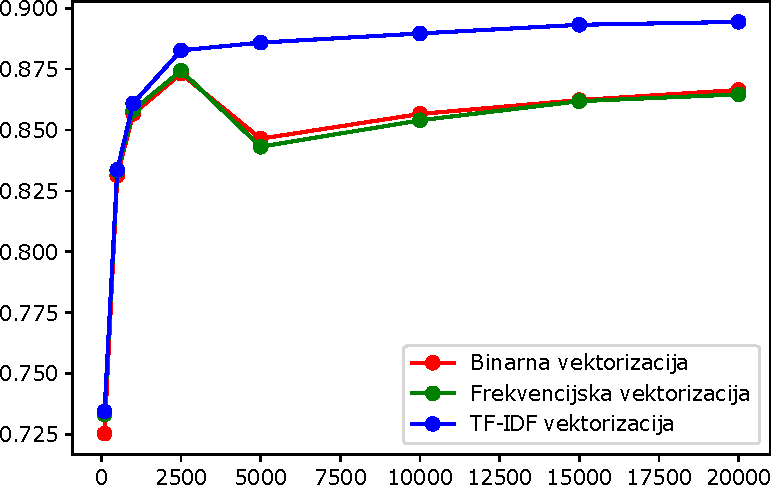
\includegraphics{vec_model.pdf}
\caption{Točnost klasifikacije u odnosu na model vektorizacije i dimenziju vektora značajki}
\label{fig:vecmodel}
\end{figure}

Sa slike \ref{fig:vecmodel} može se vidjeti kako model TF-IDF daje najbolje rezultate.
Posebice je vidljiva razlika između modela TF-IDF i ostala dva modela za vektore značajki većih
dimenzija.
Iznenađujuć je odnos između binarnog i frekvencijskog modela. 
Oba modela postižu slične rezultate, no za neke dimenzije binarni model se ponaša bolje od frekvencijskog.

\subsection{Izbor n-grama}
Nakon izbora modela i dimenzije vektora značajki, slijedi odabir raspona $n$-grama.
Dosad u testovima su korišteni unigrami, no cilj ovog testa je provjeriti kako odabir
n-grama utječe na točnost klasifikatora.
Osim klasifikatora koji koristi samo jednu vrijednost parametra $n$, može se izgraditi i klasifikator
koji primjerice koristi unigrame i bigrame. Rezultati su dani na grafu \ref{fig:grams.pdf}, 
a raspon je zadan uređenim parom (primjerice unigrami, bigrami i trigrami su zadani parom (1, 3)).

\begin{figure}
\centering
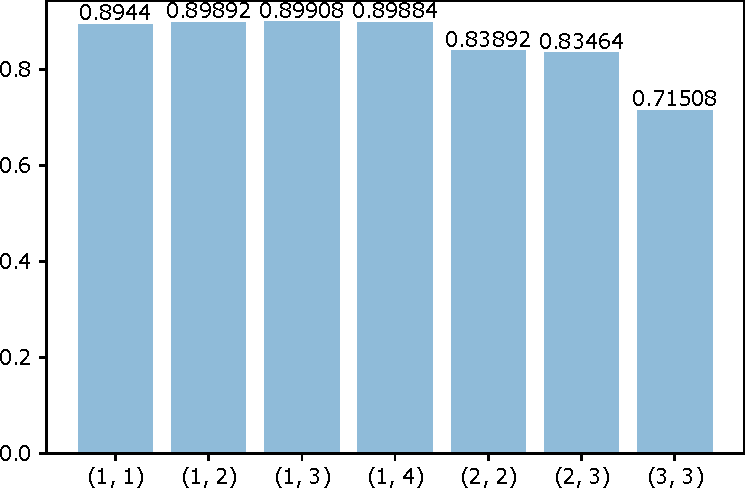
\includegraphics{grams.pdf}
\caption{Točnost klasifikatora u odnosu na izbor $n$-grama}
\label{fig:grams.pdf}
\end{figure}

Rezultati pokazuju kako unigrami samostalno ili u kombinaciji s drugim $n$-gramima daju najbolje rezultate.
Unigrami, bigrami i trigrami zajedno ostvaruju najbolji rezultat, iako su razlike neznatne.
Korištenjem složenijih struktura bez korištenja unigrama, klasifikator gubi na točnosti. 

\subsection{Analiza nositelja sentimenta}
Ne utječu svi leksemi na klasifikaciju jednako. Očekuje se da će pridjevi i prilozi nositi
sentiment dok glagoli i imenice u pravilu ne utječu na klasifikaciju.
Stoga je pametno analizirati i utjecaj leksema na klasifikaciju. Svakom leksemu pridodana je težina
dobivena optimizacijom stroja s potpornim vektorima.

\begin{table}
    \center
    \begin{tabular}{| >{\bfseries}l | l | l | >{\bfseries}l | l | l |}
    \hline
    Rank & Leksem & Težina & Rank & Leksem & Težina\\ \hline
    1 & worst & -5.097 & 11 & fails & -2.966\\ \hline
    2 & 7/10 & 3.866 & 12 & great & 2.941\\ \hline
    3 & awful & -3.821 & 13 & disappointment & -2.933\\ \hline
    4 & bad & -3.495 & 14 & 8/ & 2.857\\ \hline
    5 & excellent & 3.456 & 15 & disappointing & -2.805\\ \hline
    6 & dull & -3.418 & 16 & poor & -2.788\\ \hline
    7 & waste & -3.413 & 17 & waste\_NEG & -2.779\\ \hline
    8 & 4/10 & -3.35 & 18 & 8 & 2.714\\ \hline
    9 & boring & -3.208 & 19 & unfortunately & -2.686\\ \hline
    10 & terrible & -3.04 & 20 & amazing & 2.67\\
    \hline
    \end{tabular}
    \caption{Nositelji sentimenta koji najviše utječu na klasifikaciju}
    \label{tab:noistelji}
\end{table}

\par Tablica \ref{tab:noistelji} prikazuje dvadeset leksema koji najviše utječu na klasifikaciju.
Očekivano, tablica obiluje pridjevima. Što se tiče intenziteta sentimenta, posebno iskače riječ
\textit{worst} (hrv. \textit{najlošiji}) koja ima najveći negativni intenzitet. 
Valja uočiti kako prevladavaju nositelji negativnog sentimenta. Samo je šest pozitivnih nositelja 
sentimenta dok su ostali nositelji negativnog sentimenta. 
No, ako se uzme svih dvadeset tisuća leksema u obzir, prevladavaju nositelji pozitivnog sentimenta,
a našlo se i nekoliko riječi koje ne utječu na sentiment.
Zanimljivo je uočiti kako nekoliko leksema
poput \textit{4/10} i \textit{7/10} izrazito utječu na klasifikaciju.
Ti leksemi predstavljaju korisničke ocjene filmova te su dobar orijentir za klasifikaciju recenzija.
Interesantna je i činjenica da su recenzije po prirodi negativne budući da vrijednost slobodnog
člana $b$ iznosi $-0.048$.

\subsection{Analiza pogrešno klasificiranih primjeraka}
Nakon postupka klasifikacije, dobra je praksa pogledati i analizirati primjerke koji nisu ispravno
klasificirani. Stroj s potpornim vektorima pogriješio je u 2640 primjeraka.
Otprilike je podjednako lažno pozitivnih i lažno negativnih primjeraka.

\begin{table}
    \center
    \begin{tabular}{| L{10 cm} | l | l |}
    \hline
    Isječak recenzije & Označeno & Klasificirano \\ \hline
    ...The cinematography is badly lit, with everything looking grainy and ugly. 
    Thesound is so terrible that you can barely hear what people are saying. 
    The worst thing in this movie is the reason you're watching it-the sex.... & 1 & 0 \\ \hline
    ...Bad acting, bad direction, bad looking woman, bad sets, bad cinematography, 
    bad sound and bad sex scenes. The filmmakers should learn the difference 
    between raunchy and erotic.... & 1 & 0\\ \hline
    ...there's something compelling and memorable about it. 
    Like another commenter on the film, I saw this in childhood. 
    It's been thirty three years since 1952, but I have never forgotten the story or 
    its ridiculously cumbersome title. See it if you have the opportunity. & 0 & 1 \\  \hline
    ...HOWEVER, understand that the self-indulgent director also had many "funny gags" that 
    totally fell flat and hurt the movie. 
    His "camera tricks" weren't so much tricky but annoying and stupid. IGNORE THESE AND KEEP 
    WATCHING--it does get better. The film is fast paced, funny and worth seeing. In particular, 
    I really liked watching the acting and mugging of Max Linder--he was so expressive and funny! 
    Too bad he is virtually forgotten today. & 1 & 0\\
    \hline
    \end{tabular}
    \caption{Isječci pogrešno klasificiranih recenzija}
    \label{tab:false}
\end{table}

\par Nekoliko isječaka pogrešno klasificiranih primjeraka recenzija dano je u tablici \ref{tab:false}.
U pravilu, dojam je da klasifikator ispravno klasificira primjerke te da su tekstovi pogrešno označeni.
Zadnji primjerak prikazuje jedan od problema obrade teksta - nerazumijevanje konteksta.
Iako isječak ima nekoliko nositelja negativnog sentimenta, uz pomoć konteksta ova recenzija je 
nedvojbeno pozitivna.


\chapter{Zaključak} \label{zakljucak}
U ovom radu dan obrađen je model stroja s potpornim vektorima.
Pokazana je ideja modela, problem optimizacije te proširenje na višerazrednu klasifikaciju te regresiju.
Implementiran je dualni koordinatni spust, algoritam pogodan za učenje linearnog SVM-a.
Također, dan je uvod u problem analize sentimenta te postupak vektorizacije teksta.
Na konkretnom primjeru analize sentimenta korisničkih recenzija filmova pokazana je robusnost stroja
s potpornim vektorima.
Rezultati dobiveni klasifikacijom u pravilu su u skladu s očekivanjima.
\par Budući da je fokus u analizi sentimenta korisničkih recenzija filmova bio pronalazak pozitivnog i 
negativnog sentimenta, daljnji smjer istraživanja može biti u pravcu analize i predviđanja intenziteta
sentimenta. Valjalo bi usporediti sustav stroja s potpornim vektorima koji provodi višerazrednu klasifikaciju
te regresijskog modela za predviđanje ocjena. Valjalo bi dati i usporedbu stroja s potpornim vektorima
i nekih drugih metoda strojnog učenja te metodama dubokog učenja.
Isto tako, valjalo bi se posvetiti problemu konteksta u analizi sentimenta te analizi sentimenta na razini
rečenica ili značajki. Pogodan problem koji se dotiče konteksta i razini značajki su političke rasprave.
\par Na kraju valja zaključiti kako model stroja s potpornim vektorima je jedan od najboljih modela za
binarnu klasifikaciju podataka.
Njegova robusnost na pretreniranost, jezgreni trikovi koji rješavaju problem linearno nerazdvojivih podataka
te mogućnost proširenja na probleme višerazredne klasifikacije te probleme regresije čine ga dobrim izborom
za većinu problema iz domene strojnog učenja.

\bibliography{literatura}
\bibliographystyle{fer}

\begin{sazetak}
Stroj s potpornim vektorima (engl. Support Vector Machine, SVM) vrlo je općenit postupak koji 
omogućava rješavanje klasifikacijskih problema te problema funkcijske regresije. 
Isti je u praksi primjenjivan na niz praktičnih problema. 
U okviru završnog rada proučen je i opisan stroj s potpornim vektorima. 
Također, ostvarena je njegova programska implementacija kao i implementacija prikladnog postupka učenja 
istoga. Proučena je primjena stroja s potpornim vektorima na rješavanje problema analize sentimenta 
korisničkih recenzija te je ispitan rad algoritma na korisničkim recenzijama filmova.
Rezultati dobiveni klasifikacijom recenzija su prikazani i analizirani. 


\kljucnerijeci{stroj s potpornim vektorima, analiza sentimenta, klasifikacija, SVM, strojno učenje, 
regresija, dualni koordinatni spust}
\end{sazetak}

% TODO: Navedite naslov na engleskom jeziku.
\engtitle{Application of Support Vector Machine for Users' Reviews Sentiment Analysis}
\begin{abstract}
Support vector machines (SVM) are supervised learning models which can solve regression and classification
problems. This thesis describes and analyses the support vector machine model.
Moreover, dual coordinate descent, an optimization algorithm for solving linear SVM is implemented.
In the second part of the thesis, a brief introduction to sentiment analysis is given. 
In the last part of the thesis, film reviews are classified using linear support vector machine and 
the results are interpreted.


\keywords{Support Vector Machine, SVM, Sentiment Analysis, Classification, Regression, Machine Learning, 
Dual Coordinate Descent}
\end{abstract}

\end{document}
